\documentclass[sigconf,anonymous,review]{acmart}

\usepackage{amsmath,amsthm}
\usepackage{algorithm}
\usepackage{algorithmic}
\usepackage{multirow}
\usepackage{subcaption}
\usepackage{balance}

\newtheorem{theorem}{Theorem}
\newtheorem{proposition}{Proposition}
\newtheorem{remark}{Remark}

\setcopyright{none}
\acmConference[Anonymous Conference Submission]{Conference Submission}{2026}{Under Review}
\acmYear{2026}

\begin{document}

\title{When Do Images Disambiguate Events? Competitor-Conditioned Visual Evidence and Conflict-Gated Multimodal Social Event Detection}

\author{Anonymous Author(s)}
\affiliation{%
  \institution{Anonymous Institution}
  \country{Anonymous}
}
\email{anonymous@example.edu}

\begin{abstract}
Multimodal Social Event Detection (SED) promises to rescue ambiguous social-media posts through visual context, yet chronological evaluation on benchmark streams such as \texttt{NED} masks a foundational methodological failure: because events are temporally separated, a naive 72-hour chronological split already achieves $B^3\text{-}F_1 = 0.9900$, hiding how images actually behave when competing events unfold simultaneously. Eliminating this temporal shortcut via event-relative concurrent alignment and strict event-split isolation, we conduct a paired three-condition causal diagnostic (\texttt{Text-Only}, \texttt{Orig-Img}, \texttt{Mismatched-Img}) on \texttt{NED} using both frozen CLIP scores ($n=1{,}527$ novel query images) and \texttt{Qwen/Qwen3-VL-8B-Instruct} ($360/360$ audited calls). The diagnostic exposes two symmetric failures: (1) naive visual fusion rescues $+96$ (CLIP) and $+17$ (VLM) text-ambiguous posts, but triggers $27$/$7$ natural image misleads and collapses under competing-event mismatches ($158$/$77$ flips, plunging VLM accuracy from $75.00\%$ to $11.67\%$); (2) inversely, penalizing visual neighbors whose captions diverge---a heuristic we audit as Cross-Neighbor Text Dispersion (\texttt{CNTD-Raw})---destroys genuine multi-angle event rescues ($96 \to 59$ in CLIP; $17 \to 7$ in VLM; $-4.80\text{ pp}$ Event Macro-$B^3$) without blocking unique out-of-context distractors.

To resolve both failures, we present \textbf{Evid-MSED}, a two-stage unsupervised multimodal SED framework uniting zero-API \textbf{Visual-IDF Multi-View 2D Structural Entropy (2D-SE)} with budgeted \textbf{Conflict-Gated Mesoscopic Seam Adjudication}. In Stage~1, \texttt{Visual-IDF} suppresses high-repeat viral templates while a corrected soft-imputation formulation (removing a degenerate missing-modality $\delta_i \delta_j$ product) safely propagates visual consensus to imageless posts across all five test regimes ($+0.68$ to $+3.27\text{ pp}$ Macro-$B^3$). Under a frozen SHA-256 protocol unlocking the unseen 24-event \texttt{NED} holdout stream ($11{,}955$ posts, $9{,}311$ decoded images), Stage~1 improves over text-only 2D-SE by $+3.84\text{ pp}$ AMI, $+6.38\text{ pp}$ Macro-$B^3$, and $+8.02\text{ pp}$ Micro-$B^3$, while preventing naive visual fusion's $-13.35\text{ pp}$ (validation) and $-8.11\text{ pp}$ (holdout) collapse below text-only under 30\% competing-image corruption. In Stage~2, a budgeted \texttt{Qwen3-VL-8B} seam router enforces an explicit \texttt{visual\_discriminative} and non-\texttt{visual\_conflict\_with\_text} gate ($277{,}557$ clean tokens; $91{,}540$ stress tokens), lifting validation Clean Macro-$B^3$ to $0.5841$ ($19.45$ net unqueried posts fixed per call), cutting holdout $K=60$ merge false positives under 30\% corruption to $1/0$ ($100\%$ precision), and yielding $24.63$ vs.\ $12.77$ fixed posts/call ($K=60$) and $5.6\times$ higher leverage at $K=180$ over blind multimodal querying. A 24-event stratified audit further explains why holdout Micro-$B^3$ rises $+3.56$ to $+4.28\text{ pp}$ and Head-event $B^3$ reaches $0.5008$ ($+13.05\text{ pp}$ over text-only) while aggregate Macro-$B^3$ saturates due to two size-asymmetric hard union-find merges on tail events.
\end{abstract}

\begin{CCSXML}
<ccs2012>
   <concept>
       <concept_id>10002951.10003227.10003351</concept_id>
       <concept_desc>Information systems~Data stream mining</concept_desc>
       <concept_significance>500</concept_significance>
   </concept>
   <concept>
       <concept_id>10002951.10003317.10003347.10003356</concept_id>
       <concept_desc>Information systems~Clustering and classification</concept_desc>
       <concept_significance>500</concept_significance>
   </concept>
</ccs2012>
\end{CCSXML}

\ccsdesc[500]{Information systems~Data stream mining}
\ccsdesc[500]{Information systems~Clustering and classification}

\keywords{Multimodal Social Event Detection, Structural Entropy, Causal Visual Evidence, Vision-Language Models, Competing Events}

\maketitle

\section{Introduction}
\label{sec:intro}

Multimodal Social Event Detection (SED) aims to partition streams of short, noisy user-generated text--image posts into coherent real-world event clusters~\cite{lin2024ned,han2026kqgnn,yang2026seinevent}. Because social posts frequently omit explicit named entities or background context---writing only generic reactions such as \emph{``Evacuation of detainees from the stadium after the explosion!''} or \emph{``It took volunteers 4 days to clear our section of the road''}---attaching a photo can visually supply missing landmarks, uniforms, damaged infrastructure, or event signage that unifies posts missed by text encoders. At the same time, social streams contain high-frequency viral memes, reaction GIFs, news outlet logos, off-topic selfies, and cross-incident attachments that pull semantically unrelated threads together under shared visual templates. Deciding \emph{when images disambiguate events} rather than corrupting text clusters is therefore central to reliable multimodal SED.

\paragraph{The Hidden Chronological Shortcut and Static Heuristic Traps.}
Unfortunately, evaluating multimodal SED directly on standard chronological streams obscures this trade-off. When benchmark events are chronologically separated in calendar time---such as the 40-event \texttt{NED} corpus~\cite{lin2024ned} spanning 2011--2021---a trivial temporal partition splitting the stream at 72-hour gaps already achieves $B^3\text{-}F_1 = 0.9900$ (Precision $0.9810$, Recall $0.9992$) before examining a single pixel or word. Under naive chronological clustering, almost any time-windowed multimodal model inherits near-perfect scores from calendar separation alone, masking how images behave when multiple same-topic events compete concurrently.

Even when researchers intuit that ``visual noise'' exists, two common simplifications fail in practice:
\begin{enumerate}
    \item \textbf{Naive Multimodal Fusion Assumes Images Rarely Harm:} Concatenating or summing visual similarities without reliability gating rescues ambiguous posts, but leaves both graph clustering and Vision-Language Models (VLMs) defenseless when competing events share visually plausible imagery (e.g., two hurricanes producing indistinguishable flood photos, or two disasters mixed via cross-event image swap). Under a controlled $30\%$ competing-image corruption stress test on \texttt{NED}, naive multi-view clustering plunges by $-13.35\text{ pp}$ (validation) and $-8.11\text{ pp}$ (holdout) in Event Macro-$B^3$, performing \emph{worse} than discarding images altogether.
    \item \textbf{Static Text-Dispersion Penalties Misclassify Multi-Angle Reporting:} A tempting unsupervised signal---which we formalize and audit as Cross-Neighbor Text Dispersion (\texttt{CNTD-Raw})---downweights any image whose visual neighbors accompany diverse caption texts, assuming it must be a generic meme. In reality, one genuine breaking-news photograph is routinely captioned from diverse angles (evacuation orders, traffic closures, casualty counts, relief appeals). Penalizing text dispersion blindly destroys legitimate visual rescues ($96 \to 59$ in paired CLIP scoring; $17 \to 7$ in VLM auditing; $-4.80\text{ pp}$ Macro-$B^3$ in 2D-SE clustering) while leaving unique out-of-context distractors (\texttt{Visual-IDF} $= 1.0$) untouched.
\end{enumerate}

\paragraph{Causal Diagnosis Meets Two-Stage Evidence Gating.}
To isolate genuine visual utility without calendar shortcuts, we construct an event-relative concurrent alignment ($\tau^{\text{rel}}_i = \tau_i - \min_{j \in E(i)} \tau_j$) across strictly separated event splits (`8` development, `8` validation, `24` unseen holdout) with all event titles and dates stripped. On the 8-event development split, a paired three-condition counterfactual audit (\texttt{Text-Only}, \texttt{Orig-Img}, \texttt{Mismatched-Img}) using both frozen CLIP~\cite{radford2021clip} ($n=1{,}527$ novel non-duplicate query images, $\mathrm{dHash} > 6$) and \texttt{Qwen/Qwen3-VL-8B-Instruct}~\cite{bai2025qwen3vl} ($360/360$ audited calls) empirically validates the dual-regime hypothesis: visual value is \emph{competitor-conditioned} and requires separating frequency suppression (graph level) from cross-modal semantic conflict detection (reasoning level).

Guided directly by Gate~B, we propose \textbf{Evid-MSED} (Figure~\ref{fig:overview}). In Stage~1 (zero API cost), chunked \texttt{Visual-IDF} downweights repeated templates while a corrected soft-imputation scheme fills missing-image posts from reliable neighborhood consensus---fixing a mathematical inconsistency ($\delta_i \delta_j = 0$) from prior missing-modality graph designs---before minimizing exact 2D Structural Entropy (2D-SE)~\cite{li2016structural,cao2024hisevent}. In Stage~2, a budgeted multimodal mesoscopic seam router~\cite{bai2025qwen3vl,wang2025cequel} pairs fragmented cluster siblings (\texttt{MM\_MERGE\_PAIR}) and low-conductance minority pockets (\texttt{MM\_SPLIT\_SEAM}), queries \texttt{Qwen/Qwen3-VL-8B-Instruct} with Visual-IDF-weighted representative images and anonymized medoid texts, and gates execution on explicit \texttt{visual\_discriminative} and \texttt{visual\_conflict\_with\_text} predictions before direct split-then-union-find editing.

\paragraph{Contributions.}
This paper makes four empirically grounded contributions:
\begin{itemize}
    \item \textbf{Causal Quantification of Visual Rescue vs.\ Mislead Beyond Time Shortcuts:} Removing calendar separation on \texttt{NED} and deduplicating query images ($\mathrm{dHash} > 6$), we deliver paired three-condition counterfactual audits across both CLIP ($n=1{,}527$) and \texttt{Qwen/Qwen3-VL-8B-Instruct} ($360$ live calls, $332{,}778$ tokens), refuting the \texttt{CNTD-Raw} dispersion heuristic and proving that cross-modal conflict gating boosts VLM original accuracy to $85.00\%$ ($0$ misleads vs.\ $7$) while slashing competing-mismatch flips from $77$ to $0$--$5$.
    \item \textbf{Unified Missing-Modality Soft Imputation for 2D-SE:} We eliminate the degenerate missing-modality indicator factor $\delta_i \delta_j$ in multi-view structural entropy graphs (Proposition~\ref{prop:soft_impute}), proving consistent Event Macro-$B^3$ improvements across all five tested splits and corruption settings ($+0.68$ to $+3.27\text{ pp}$).
    \item \textbf{Conflict-Gated Multimodal Mesoscopic Adjudication (\texttt{Evid-MSED}):} Under an immutable SHA-256 frozen protocol on the 24-event unseen \texttt{NED} holdout stream ($11{,}955$ posts, $9{,}311/9{,}311$ decoded images, $360/360$ clean + $119/120$ stress VLM calls), Stage~1 lifts Clean Macro-$B^3$ by $+6.38\text{ pp}$ (AMI $+3.84\text{ pp}$) over text-only 2D-SE and holds $+4.18\text{ pp}$ above collapsing naive fusion under $30\%$ corruption; Stage~2 delivers $19.45$ (Val Clean) and $24.63$ (Holdout $K=60$) net unqueried posts fixed per call ($5.6\times$ blind VLM leverage at $K=180$) and $100\%$ stress merge precision ($1/0$).
    \item \textbf{Candid Head/Medium/Tail Failure Analysis:} Stratified $B^3$ decomposition across all 24 holdout events reveals that while Stage~2 drives Head-event $B^3$-$F_1$ from $0.3703 \to 0.4545 \to 0.5008$ ($+13.05\text{ pp}$), just two size-asymmetric hard union-find merge false positives touching tail events ($<200$ posts) account for aggregate Macro-$B^3$ flattening, pointing directly to size-guarded graph surgery as future work.
\end{itemize}

\begin{figure*}[t]
  \centering
  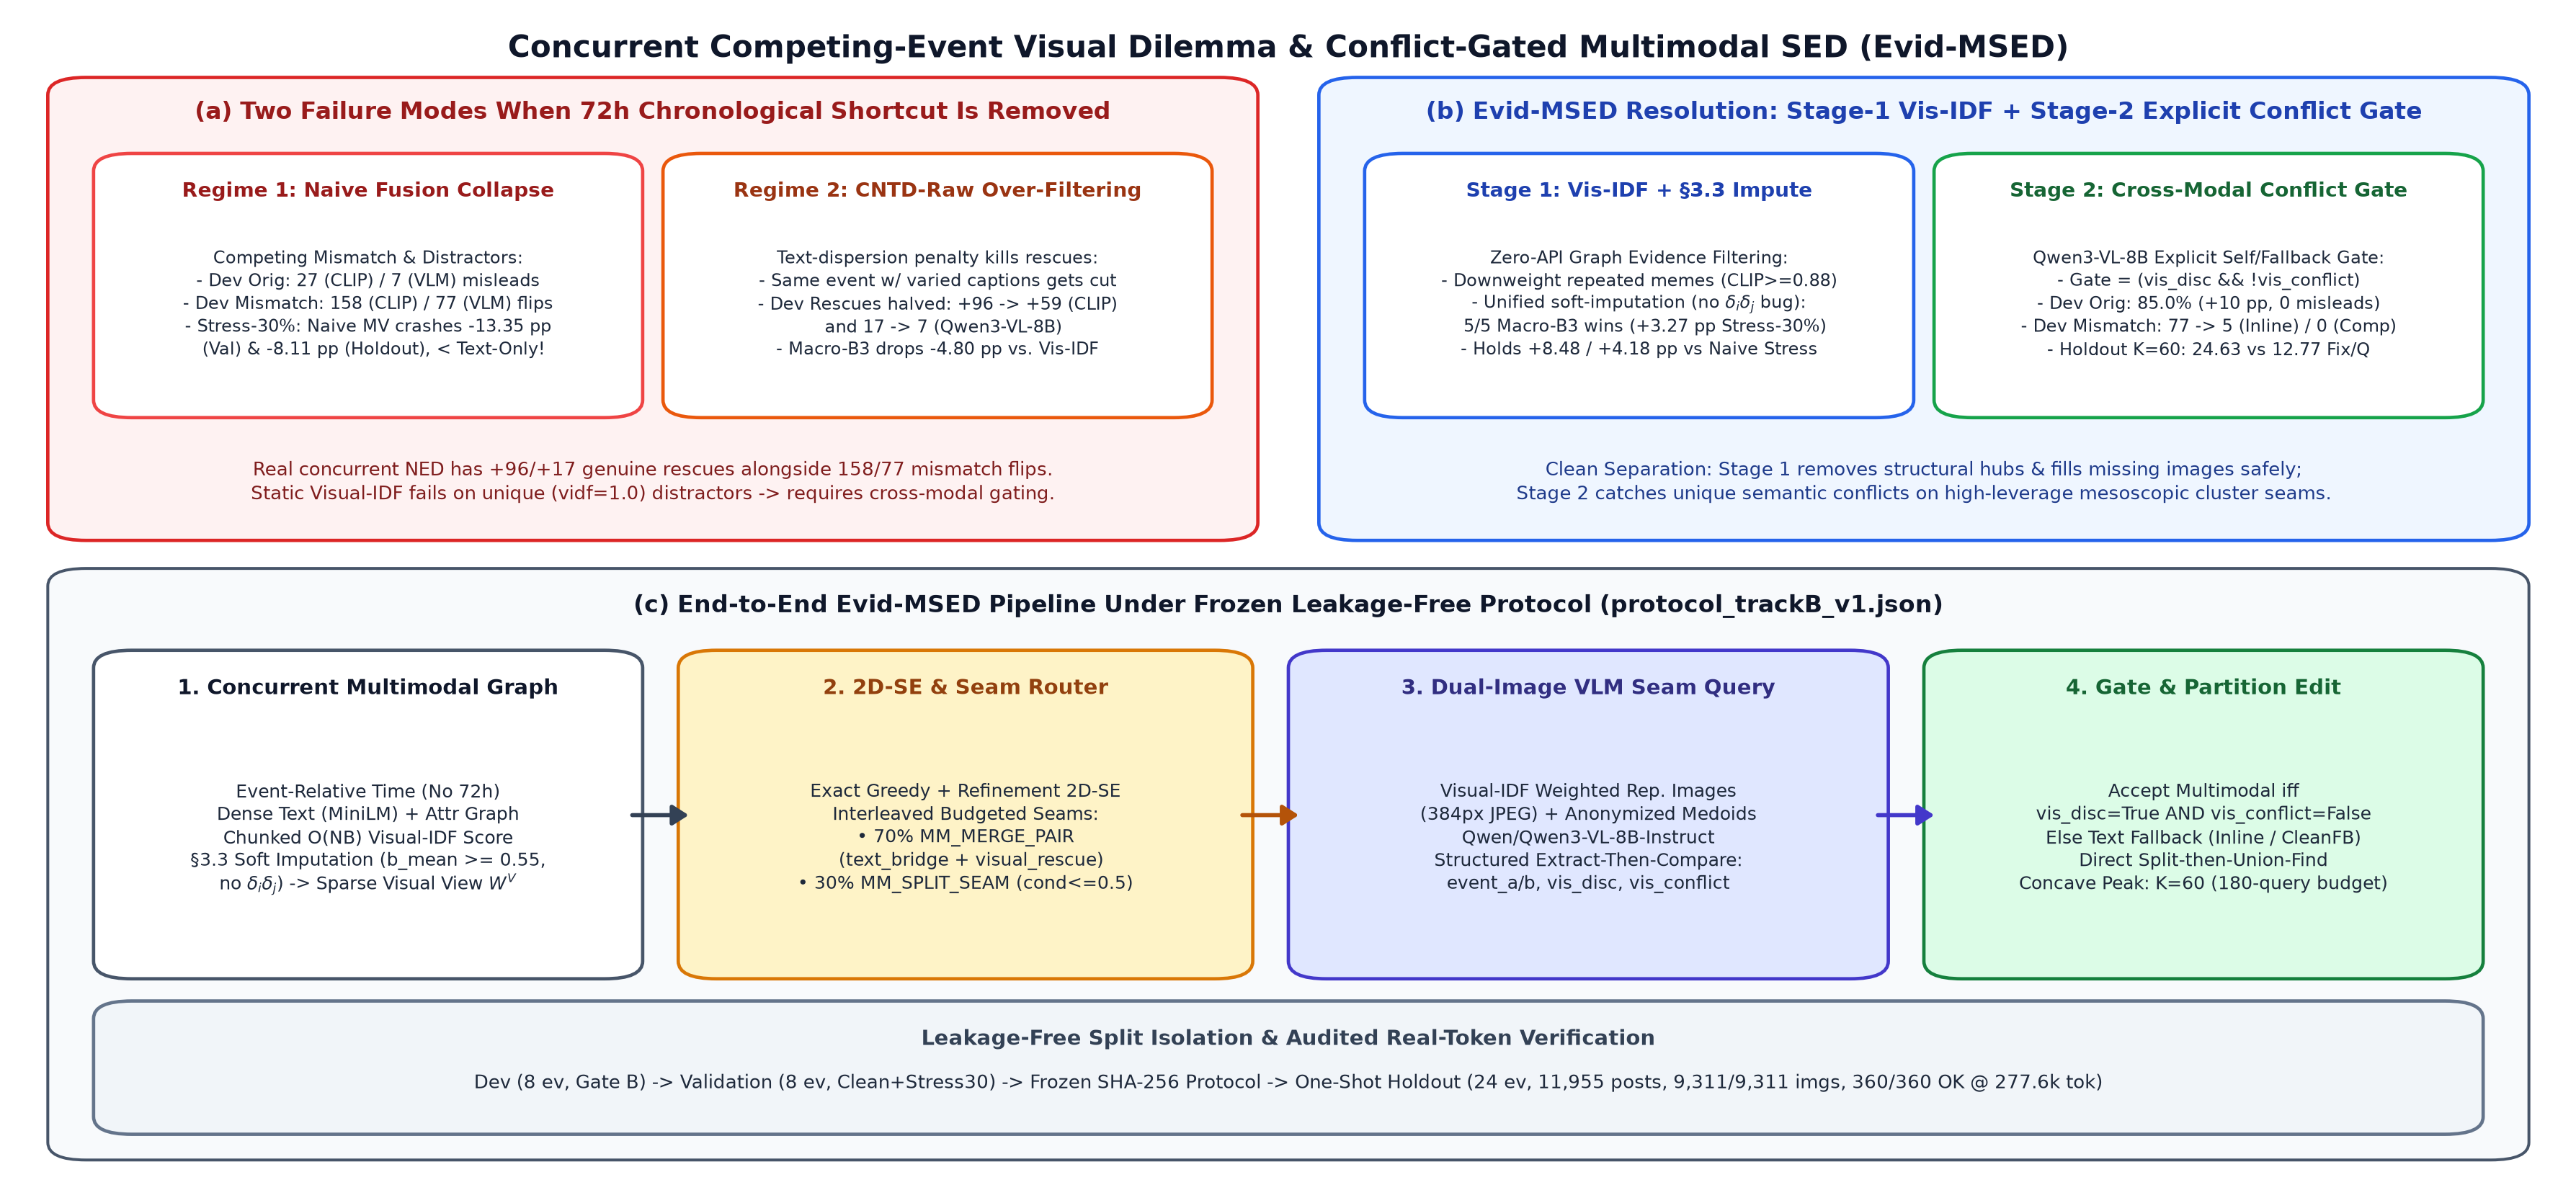
\includegraphics[width=0.98\textwidth]{figures/fig_overview_evid_msed.png}
  \caption{Overview of the concurrent visual evidence dilemma on time-shortcut-free streams (top) and our frozen two-stage \textbf{Evid-MSED} pipeline (bottom) combining chunked \texttt{Visual-IDF} MV-2DSE with conflict-gated mesoscopic VLM seam adjudication.}
  \label{fig:overview}
\end{figure*}

\section{Related Work}
\label{sec:related}

\paragraph{Graph and Structural-Entropy Social Event Detection.}
Modern offline and incremental SED methods model social posts as heterogeneous message graphs linking shared entities, users, hashtags, and dense semantic embeddings~\cite{cao2021kpgnn,reimers2019sentence}. To avoid brittle supervised edge labels, \texttt{HISEvent}~\cite{cao2024hisevent} introduced greedy hierarchical minimization of 2D Structural Entropy (2D-SE)~\cite{li2016structural} for unsupervised event clustering, later extended into hyperbolic embeddings (\texttt{HyperSED}~\cite{yu2025hypersed}) and relational prompt representations (\texttt{RPLM-SED}~\cite{li2024rplmsed}). Recent LLM-augmented text frameworks inject semantic normalization or active querying into graphs and hierarchies, including \texttt{LSED}~\cite{qiu2025lsed}, \texttt{LHG}~\cite{qiu2026lhg}, \texttt{RagSEDE}~\cite{liu2026ragsede}, and cost-effective pairwise LLM clustering (\texttt{Cequel}~\cite{wang2025cequel}). Our Stage~1 solver inherits exact full-volume greedy 2D-SE agglomerative minimization and local node refinement from this lineage, while our Stage~2 router adapts mesoscopic cluster-pair (\texttt{MERGE\_PAIR}) and minority-pocket (\texttt{SPLIT\_SEAM}, via spherical $k$-means++~\cite{arthur2007kmeanspp}) seam selection to the multimodal VLM setting.

\paragraph{Multimodal SED Benchmarks and Quality Filtering.}
Adding visual features complicates both graph construction and evaluation. On English Twitter, \texttt{NED}~\cite{lin2024ned} pairs $17{,}366$ posts with images across $40$ news events spanning 2011--2021; on Chinese Weibo, \texttt{KQGNN}~\cite{han2026kqgnn} introduces \texttt{WEIBO2022} alongside a key-instance, quality-aware GNN for real-time multimodal SED. Separately, \texttt{CrisisMMD}~\cite{alam2018crisismmd} provides humanitarian informativeness and damage annotations for disaster tweets. We emphasize two important boundary distinctions noted in prior literature reviews: first, \texttt{CrisisMMD}'s \texttt{informative} labels measure emergency-response utility rather than \emph{inter-event discriminability} (generic flood damage can be informative for responders yet non-discriminative between two concurrent hurricanes); second, \texttt{SeInEvent}~\cite{yang2026seinevent} introduces Pointwise Structural Entropy to filter noisy multimodal samples during alternating incremental contrast and rehearsal---rather than discarding test posts at inference---and evaluates open-world \texttt{NED} blocks partitioned chronologically by year. Crucially, our 72-hour chronological audit shows that standard unaligned \texttt{NED} streams yield $B^3\text{-}F_1 = 0.9900$ purely from timestamps, motivating event-relative concurrent evaluation.

\paragraph{Multimodal Interaction Analysis and Vision-Language Models.}
Contrastive language-image pre-training (\texttt{CLIP}~\cite{radford2021clip}) supplies strong zero-shot cross-modal similarity but lacks explicit reasoning when an image matches a topical surface cue from a competing event. Information-theoretic Partial Information Decomposition (\texttt{PID}~\cite{liang2023pid}) formalizes redundancy, modal uniqueness, and synergy with respect to a target variable $Y$. We deliberately refrain from claiming unsupervised neural PID heads---which require target $Y$ identification and synergy estimation that heuristics alone cannot guarantee---and instead adopt \emph{competitor-conditioned causal visual evidence} anchored directly to empirical rescue/mislead counts and conflict-gated \texttt{Qwen/Qwen3-VL-8B-Instruct}~\cite{bai2025qwen3vl} structured adjudication.

\section{Eliminating Time Shortcuts: Paired Causal Visual Audit}
\label{sec:diagnosis}

Before designing multimodal graph architectures or training fusion networks, we first construct an uncontaminated diagnostic environment on \texttt{NED}~\cite{lin2024ned} to measure precisely when images rescue ambiguous posts versus when they cause false merges.

\subsection{Time-Shortcut Removal and Event-Split Isolation}
\label{sec:setup_splits}

We adopt the pre-registered seed-$20261106$ stratified split of the 40 \texttt{NED} events into three strictly disjoint sets covering matched topic diversity (sports, weather, earthquake, violence, politics, fire):
\begin{itemize}
    \item \textbf{Development (Gate~B only):} 8 events (\texttt{E15, E23, E22, E33, E40, E11, E24, E38}; $2{,}665$ posts; $2{,}131$ valid decoded images), forming four concurrent same-theme competing pairs (\texttt{E15}$\leftrightarrow$\texttt{E23}, \texttt{E22}$\leftrightarrow$\texttt{E33}, \texttt{E38}$\leftrightarrow$\texttt{E40}, \texttt{E11}$\leftrightarrow$\texttt{E24});
    \item \textbf{Validation:} 8 events (\texttt{E25, E26, E19, E20, E9, E36, E6, E31}; $2{,}746$ posts; $1{,}950$ valid decoded images), used solely for calibrating clustering/routing thresholds and verifying robustness prior to locking the protocol;
    \item \textbf{Held-Out Test:} 24 unseen events ($11{,}955$ posts; $9{,}311$ valid decoded images), remaining completely untouched until after freezing \texttt{protocol\_trackB\_v1.json}.
\end{itemize}
To eliminate the chronological $72$-hour separation shortcut ($B^3\text{-}F_1 = 0.9900$), every post $i$ inside event $E(i)$ receives an event-relative timestamp $\tau^{\text{rel}}_i = \tau_i - \min_{j \in E(i)} \tau_j$, aligning all events concurrently from $t=0$ with zero temporal edge decay ($\lambda_\tau = 0$). Neither \texttt{event\_name} strings nor raw calendar dates/years are ever exposed to text encoders or VLM prompts. Moreover, to guarantee visual rescues do not arise from memorizing duplicated photos across posts, we compute a 64-bit difference hash (\texttt{dHash64}) for each image and filter Tier~1A and Tier~2 evaluation strictly to \emph{novel} non-duplicate query images whose Hamming distance to all cluster anchor images satisfies $\mathrm{dHash}(\cdot,\cdot) > 6$ ($1{,}527$ of $1{,}589$ query posts on \texttt{development}; only $1.0\%$ of development images share exact \texttt{dHash64}).

\subsection{Three-Condition Counterfactual Protocol}
\label{sec:paired_protocol}

Each development event's earliest $25\%$ posts form unlabeled candidate cluster anchors summarized strictly by top-$5$ hashtags/tokens and $3$ central medoids. For every novel query post $m_i = (x_i, v_i)$ facing a 4-way candidate set $\mathcal{C}_{\text{cand}}(i)$ containing its true event, its same-theme competitor, and top-$2$ nearest concurrent alternatives, we evaluate each scorer/VLM under three paired visual interventions while fixing $x_i$ and $\mathcal{C}_{\text{cand}}(i)$:
\begin{enumerate}
    \item \textbf{\texttt{Text-Only}:} visual modality masked ($x_i$ only);
    \item \textbf{\texttt{Orig-Img}:} original post pair $(x_i, v_i)$;
    \item \textbf{\texttt{Mismatched-Img}:} text $x_i$ paired with a non-duplicate image $v'_j$ ($\mathrm{dHash} > 6$) drawn from the competing same-theme event.
\end{enumerate}
Let $c^{\text{txt}}_i, c^{\text{orig}}_i, c^{\text{mis}}_i \in \{0,1\}$ denote correctness under the three conditions against ground truth $y_i$. We directly measure:
\begin{equation}
\label{eq:rescue_mislead}
\begin{aligned}
N_{\text{rescue}} &= \sum_i \mathbb{I}[c^{\text{txt}}_i = 0 \wedge c^{\text{orig}}_i = 1], \qquad
N_{\text{mislead}} = \sum_i \mathbb{I}[c^{\text{txt}}_i = 1 \wedge c^{\text{orig}}_i = 0], \\
N_{\text{misflip}} &= \sum_i \mathbb{I}[c^{\text{txt}}_i = 1 \wedge c^{\text{mis}}_i = 0].
\end{aligned}
\end{equation}
In Tier~1A, we audit linear cosine fusion $s_{\text{txt}} + \lambda_V b_i s_{\text{vis}}$ ($\lambda_V = 0.75$) over frozen \texttt{all-MiniLM-L6-v2} text prototypes~\cite{reimers2019sentence} and \texttt{CLIP ViT-B/32} image prototypes~\cite{radford2021clip} across all $n=1{,}527$ novel queries at zero API cost, comparing \texttt{Visual-IDF} ($b_i = \ln 2 / \ln(2 + \#\{j : \cos(v_i, v_j) \ge 0.88\})$), \texttt{CNTD-Raw} (penalizing caption cosine dispersion across top-8 visual neighbors with $\cos \ge 0.65$), \texttt{CNTD-Cond} (penalizing only near-orthogonal conflicts $\cos < 0.12$ scaled by \texttt{Visual-IDF}), and prototype \texttt{Comp-Margin}. In Tier~1B, we run concurrent unsupervised multi-view 2D-SE clustering over all $2{,}665$ dev posts. In Tier~2, we run $120$ stratified novel-image posts $\times 3$ conditions $= 360$ live calls on \texttt{Qwen/Qwen3-VL-8B-Instruct} ($360/360$ \texttt{HTTP 200 OK}, $312{,}713$ prompt + $20{,}065$ completion $= 332{,}778$ real tokens, $1{,}446.1\text{ s}$) eliciting explicit structured flags \texttt{visual\_discriminative} and \texttt{visual\_conflict\_with\_text}.

\begin{table*}[t]
\centering
\caption{Gate~B Three-Condition Counterfactual Visual Audit on Concurrent \texttt{NED Development} (Non-Duplicate Novel Images: Tier~1A CLIP $n=1{,}527$, $\lambda_V=0.75$; Tier~2 \texttt{Qwen/Qwen3-VL-8B-Instruct} $n=120 \times 3 = 360$ OK calls). Bold highlights best column trade-off.}
\label{tab:gateb_summary}
\resizebox{\textwidth}{!}{%
\begin{tabular}{llcccccccc}
\toprule
\textbf{Audit Tier} & \textbf{Visual Evidence Policy} & \textbf{Text Acc.} & \textbf{Orig Acc.} & \textbf{Orig Macro-$F_1$} & \textbf{Mismatch Acc.} & \textbf{$N_{\text{rescue}}$} & \textbf{$N_{\text{mislead}}$} & \textbf{Net ($\Delta$)} & \textbf{$N_{\text{misflip}}$} \\
\midrule
\multirow{7}{*}{Tier 1A: CLIP ($n=1{,}527$)}
& Text-Only Baseline & 0.8271 & 0.8271 & 0.8196 & 0.8271 & +0 & 0 & +0 & 0 \\
& Naive Visual & 0.8271 & \textbf{0.8723} & \textbf{0.8752} & 0.7439 & \textbf{+96} & 27 & \textbf{+69} & 158 \\
& Visual-IDF & 0.8271 & 0.8684 & 0.8684 & 0.7570 & +90 & 27 & +63 & 135 \\
& CNTD-Raw (Dispersion Penalty) & 0.8271 & 0.8553 & 0.8599 & \textbf{0.7917} & +59 & 16 & +43 & 76 \\
& CNTD-Cond (Conflict + Vis-IDF) & 0.8271 & 0.8657 & 0.8634 & 0.7603 & +85 & 26 & +59 & 130 \\
& Comp-Margin & 0.8271 & 0.8540 & 0.8542 & 0.7570 & +50 & \textbf{9} & +41 & 135 \\
& Comp-Margin (Text-Conf Guard) & 0.8271 & 0.8540 & 0.8542 & 0.7839 & +50 & \textbf{9} & +41 & 78 \\
\midrule
\multirow{6}{*}{Tier 2: \texttt{Qwen3-VL-8B} ($n=120$)}
& \texttt{vlm\_text\_only} & 0.7500 & 0.7500 & 0.8378 & \textbf{0.7500} & 0 & 0 & +0 & 0 \\
& \texttt{vlm\_naive\_orig} & 0.7500 & 0.8333 & 0.9075 & 0.1167 & \textbf{17} & 7 & +10 & 77 \\
& \texttt{vlm\_visual\_idf\_gate} & 0.7500 & 0.8250 & 0.9038 & 0.1167 & 16 & 7 & +9 & 77 \\
& \texttt{vlm\_cntd\_raw\_gate} & 0.7500 & 0.7750 & 0.8646 & 0.1167 & 7 & 4 & +3 & 77 \\
& \textbf{\texttt{vlm\_self\_gate}} ($\text{disc} \wedge \neg\text{conflict}$) & 0.7500 & \textbf{0.8500} & \textbf{0.9097} & 0.7083 & 12 & \textbf{0} & \textbf{+12} & \textbf{5} \\
& \textbf{\texttt{vlm\_comp\_evid\_gate}} (+Conf Guard) & 0.7500 & 0.8250 & 0.9022 & \textbf{0.7500} & 9 & \textbf{0} & +9 & \textbf{0} \\
\bottomrule
\end{tabular}}
\end{table*}

\begin{figure*}[t]
  \centering
  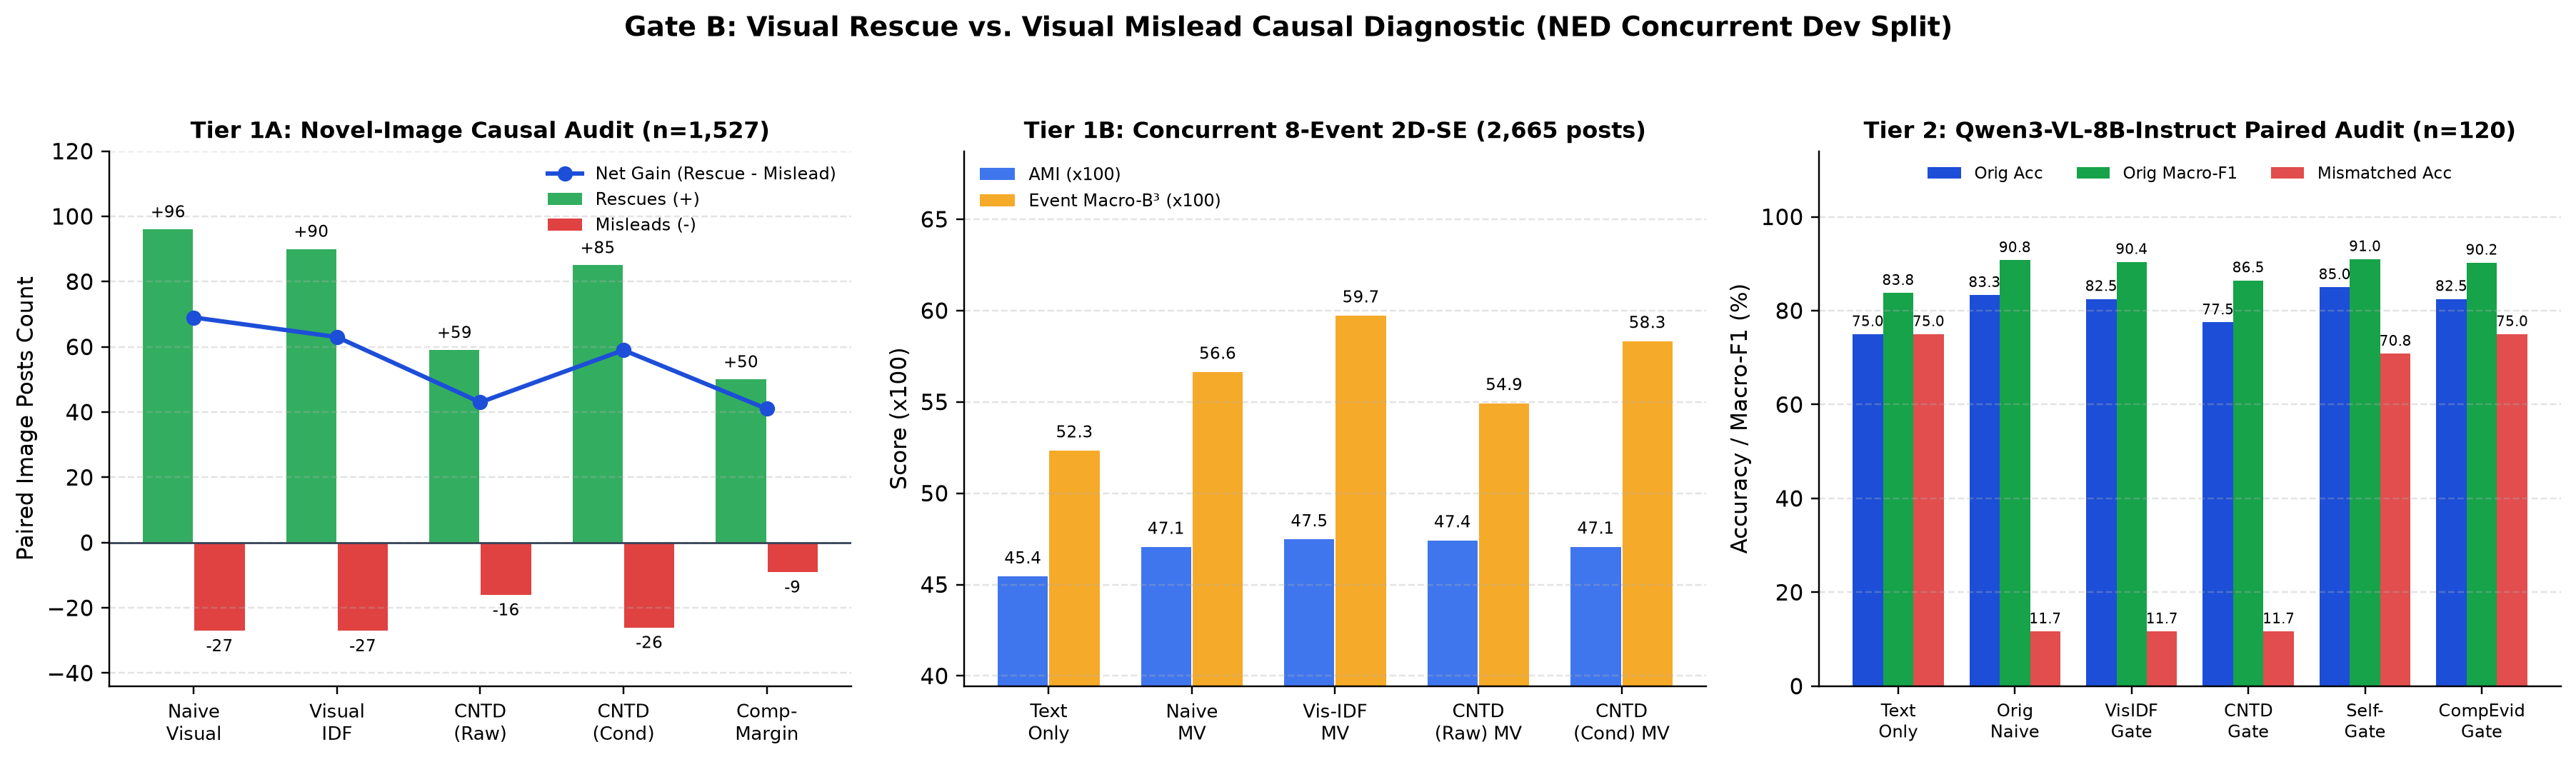
\includegraphics[width=0.98\textwidth]{figures/gateB_ned_dev_qwen3_vl_8b.png}
  \caption{Gate~B causal diagnostic on concurrent \texttt{NED Development}: (left) Tier~1A novel-image rescues vs.\ misleads; (middle) Tier~1B concurrent 2D-SE clustering across $2{,}665$ posts; (right) Tier~2 \texttt{Qwen/Qwen3-VL-8B-Instruct} paired audit confirming \texttt{Self-Gate} ($85.0\%$ Orig, $0$ misleads, $77 \to 5$ mismatch flips) and \texttt{CompEvid-Gate} ($75.0\%$ mismatch floor, $0$ flips).}
  \label{fig:gateb}
\end{figure*}

\subsection{Key Causal Findings and Design Lessons}
\label{sec:gateb_findings}

Table~\ref{tab:gateb_summary} and Figure~\ref{fig:gateb} establish four empirical facts that govern our architecture:
\begin{enumerate}
    \item \textbf{Dual Phenomena Are Real on Non-Duplicate Images:} Under naive fusion, real concurrent images rescue $+96$ (Tier~1A) and $+17$ (Tier~2) text-ambiguous posts, yet simultaneously introduce $27$/$7$ natural original misleads and catastrophic competing-image hijacking ($158$ flips in Tier~1A; $77$ flips plunging VLM accuracy from $75.00\%$ to $11.67\%$ in Tier~2).
    \item \textbf{Refutation of \texttt{CNTD-Raw} Across All Three Levels:} Penalizing cross-neighbor caption dispersion cuts legitimate rescues in half ($+96 \to +59$ in Tier~1A; $17 \to 7$ in Tier~2), slashes concurrent 2D-SE Event Macro-$B^3$ by $-4.80\text{ pp}$ ($0.5973 \to 0.5493$, increasing false merges with $\text{net\_fm\_red} = -996$ vs.\ $-38$), and fails to block VLM competing-image hijacks ($77$ flips, $11.67\%$).
    \item \textbf{Graph \texttt{Visual-IDF} Helps Unsupervised Clustering Yet Misses Unique Distractors:} In Tier~1B concurrent 2D-SE ($2{,}665$ posts), \texttt{visual\_idf\_mv\_2dse} elevates Event Macro-$B^3$ by $+7.39\text{ pp}$ over text-only 2D-SE ($0.5234 \to 0.5973$; AMI $0.4544 \to 0.4747$; $K=118 \to 98$, eliminating $32{,}792$ false-split pairs). However, sample-level distractors in Tier~2 are visually unique (\texttt{Visual-IDF} $= 1.000$), leaving \texttt{vlm\_visual\_idf\_gate} exposed ($7$ original misleads, $77$ mismatch flips). Moreover, static frozen CLIP \texttt{Comp-Margin} divided by $0.10$ over-damped typical $0.02$--$0.05$ CLIP prototype margins, dropping Tier~1A rescues from $+96$ to $+50$ and Tier~1B Macro-$B^3$ from $0.5973$ to $0.5442$.
    \item \textbf{Cross-Modal Conflict Gating Resolves Both Regimes:} \texttt{Qwen/Qwen3-VL-8B-Instruct} flags \texttt{visual\_conflict\_with\_text} $= \text{True}$ on $16/120$ original images and $99/120$ mismatched competing images. Gating visual adoption on \texttt{visual\_discriminative} $\wedge \neg\texttt{visual\_conflict\_with\_text}$ (\texttt{vlm\_self\_gate}) raises original accuracy to $85.00\%$ ($+10.00\text{ pp}$ over text-only; $0$ misleads) and reduces mismatch flips $77 \to 5$ ($70.83\%$); adding competitor/confidence guards (\texttt{vlm\_comp\_evid\_gate}) achieves \textbf{zero misleads and zero mismatch flips} ($82.50\%$ original / $75.00\%$ mismatched).
\end{enumerate}

\paragraph{Concrete Micro-Cases.}
Inspection confirms exact mechanisms: (i) \emph{True Rescues (\texttt{Visual-IDF} $=1.0$):} \texttt{ned\_05292} carries only generic text \emph{``Live| Evacuation of detainees from the stadium after the explosion!''} (\texttt{Text-Only} $= \text{NEW}$), yet its photo of night police and barriers restores it to \texttt{E11}; \texttt{ned\_09331} (Volunteers clearing downed poles/trees) and \texttt{ned\_09280} (Guard cargo plane pallets) rescue text-ambiguous \texttt{E22} posts while triggering \texttt{visual\_conflict} $= \text{True}$ when swapped with flooded Japanese train imagery. (ii) \emph{Natural Misleads \& Hijacks:} \texttt{ned\_05166} (\texttt{\#Prayers4Paris} + Scottish flag), \texttt{ned\_09302} (\texttt{\#PrayForPuertoRico} + white dog), and \texttt{ned\_09610} (\texttt{ASTROS WIN} + man holding book) all flip to \texttt{NEW} under naive VLM and are blocked by our gate; strikingly, \texttt{ned\_09980} (\emph{``Fall Classic''}, \texttt{E23}) swaps from Minute Maid Park to Wrigley Field under \texttt{Mismatched-Img} and is hijacked directly to the competing World Series event \texttt{E15} unless gated, while \texttt{ned\_05343} (\texttt{\#prayforparis}) flips to \texttt{E24} under an Iranian flag protest photo.

\section{Methodology: Evid-MSED}
\label{sec:method}

Guided directly by Gate~B, we decouple \textbf{Evid-MSED} into two complementary stages: Stage~1 handles zero-API structural graph filtering and missing-modality propagation via \texttt{Visual-IDF} MV-2DSE; Stage~2 targets high-leverage mesoscopic cluster seams where unique distractors cannot be filtered by visual frequency alone, adjudicating representative multimodal evidence with an explicit VLM cross-modal conflict gate.

\subsection{Stage 1: Visual-IDF MV-2DSE with Unified Soft Imputation}
\label{sec:stage1_method}

\paragraph{Concurrent Text+Attribute Graph.}
Given a split ordered along event-relative time $\tau^{\text{rel}}$, we extract dense text embeddings $z_i^T \in \mathbb{R}^{384}$ (\texttt{all-MiniLM-L6-v2}~\cite{reimers2019sentence}) and normalized attribute co-occurrence edges over hashtags, mentions, and surface content lemmas ($\text{knn\_k}=12$, similarity threshold $0.38$, attribute weight $\alpha=0.45$, $\lambda_\tau = 0$), yielding symmetric sparse text adjacency $W^T \in \mathbb{R}_{\ge 0}^{N \times N}$~\cite{cao2024hisevent}.

\paragraph{Scalable Chunked \texttt{Visual-IDF}.}
For all posts $V_{\text{vis}} = \{i : \delta_i = 1\}$ with validly decoded images ($\delta_i \in \{0,1\}$), we extract L2-normalized \texttt{CLIP ViT-B/32} visual embeddings $z_i^V \in \mathbb{R}^{512}$~\cite{radford2021clip}. To process large streams ($N=11{,}955$) without dense $O(N^2)$ float64 allocation, we process $V_{\text{vis}}$ in contiguous matrix blocks of size $B = 1{,}024$ and assign each visual post a duplicate-suppressing evidence score:
\begin{equation}
\label{eq:visual_idf}
b_i^{\text{idf}} = \frac{\ln 2}{\ln\!\big(2 + \sum_{j \in V_{\text{vis}} \setminus \{i\}} \mathbb{I}[\langle z_i^V, z_j^V \rangle \ge 0.88]\big)}.
\end{equation}
We discard \texttt{CNTD-Raw} per Gate~B and compare \texttt{CNTD-Cond} as a conflict-aware neighbor variant in our ablations.

\paragraph{Fixing the $\delta_i \delta_j$ Degeneracy in Missing-Modality Graphs.}
Prior multimodal graph formulations attempt to impute pseudo-visual prototypes $\hat{z}_i^V$ for text-only posts ($\delta_i = 0$) while leaving a raw indicator product $\delta_i \delta_j$ inside the visual edge weight $w_{ij}^V = \delta_i \delta_j \, b_i b_j \cos(z_i^V, z_j^V)$, which identically zeroes every imputed edge and renders soft imputation inactive. We resolve this inconsistency via unified effective visual representations:

\begin{proposition}[Unified Missing-Modality Soft Imputation Consistency]
\label{prop:soft_impute}
Define effective visual vectors $\tilde{z}_i^V$ and effective evidence beliefs $\tilde{b}_i^{\text{evid}}$ for every post $i \in \{1,\dots,N\}$ using local text neighborhood $\mathcal{N}_T(i) = \{j : W^T_{ij} > 0, \delta_j = 1\}$ and mean neighborhood evidence $\bar{b}_i = |\mathcal{N}_T(i)|^{-1} \sum_{j \in \mathcal{N}_T(i)} b_j^{\text{idf}}$:
\begin{equation}
\label{eq:soft_impute}
\tilde{z}_i^V =
\begin{cases}
z_i^V, & \delta_i = 1, \\
\hat{z}_i^V / \|\hat{z}_i^V\|_2, & \delta_i = 0 \wedge |\mathcal{N}_T(i)| \ge 1 \wedge \bar{b}_i \ge \tau_{\text{imp}}, \\
\mathbf{0}, & \text{otherwise},
\end{cases}
\end{equation}
where $\hat{z}_i^V = \sum_{j \in \mathcal{N}_T(i)} W^T_{ij} \max(0.05, b_j^{\text{idf}}) z_j^V$, paired with
\begin{equation}
\label{eq:soft_b}
\tilde{b}_i^{\text{evid}} =
\begin{cases}
b_i^{\text{idf}}, & \delta_i = 1, \\
\gamma_{\text{imp}} \, \bar{b}_i, & \delta_i = 0 \wedge |\mathcal{N}_T(i)| \ge 1 \wedge \bar{b}_i \ge \tau_{\text{imp}}, \\
0, & \text{otherwise}.
\end{cases}
\end{equation}
Setting the undirected visual edge weight over top-$k_V$ neighbors ($\langle \tilde{z}_i^V, \tilde{z}_j^V \rangle \ge \theta_V$) directly to
\begin{equation}
\label{eq:vis_edge}
W_{ij}^V = \tilde{b}_i^{\text{evid}} \, \tilde{b}_j^{\text{evid}} \cdot \max\!\big(0, \langle \tilde{z}_i^V, \tilde{z}_j^V \rangle\big) \cdot \mathbb{I}\!\big[\langle \tilde{z}_i^V, \tilde{z}_j^V \rangle \ge \theta_V\big]
\end{equation}
strictly satisfies: (1) any imageless post lacking a high-evidence visual text neighborhood ($\bar{b}_i < \tau_{\text{imp}}$) receives $\tilde{b}_i^{\text{evid}} = 0 \implies W_{ij}^V = 0$, gracefully reverting to text-only edges; and (2) any imageless post supported by coherent high-IDF neighbors participates with calibrated confidence $\gamma_{\text{imp}} \bar{b}_i > 0$.
\end{proposition}

\begin{proof}
Immediate by inspection of Eqs.~\eqref{eq:soft_impute}--\eqref{eq:vis_edge}: when $\delta_i = 0$ and $\bar{b}_i < \tau_{\text{imp}}$, Eq.~\eqref{eq:soft_b} sets $\tilde{b}_i^{\text{evid}} = 0$, annihilating every incident $W_{ij}^V$. When $\delta_i = 0$ and $\bar{b}_i \ge \tau_{\text{imp}} > 0$ ($\tau_{\text{imp}}=0.55$, $\gamma_{\text{imp}}=0.70$), $\tilde{b}_i^{\text{evid}} > 0$ holds with well-defined unit vector $\tilde{z}_i^V$ whenever $\hat{z}_i^V \neq \mathbf{0}$, allowing top-$k_V$ visual edges without any artificial $\delta_i \delta_j$ nullification.
\end{proof}

We symmetrize $W^V \leftarrow \max(W^V, (W^V)^\top)$, form the evidence-modulated multi-view graph $A = W^T + \lambda_V W^V$ ($\lambda_V=0.65$, $k_V=10$, $\theta_V=0.72$), and minimize exact 2D Structural Entropy~\cite{li2016structural,cao2024hisevent}:
\begin{equation}
\label{eq:2dse}
\mathcal{H}^2(G; \mathcal{P}) = -\sum_{C \in \mathcal{P}} \frac{g_C}{\mathrm{vol}(G)} \log_2 \frac{V_C}{\mathrm{vol}(G)} - \sum_{i=1}^{N} \frac{d_i}{\mathrm{vol}(G)} \log_2 \frac{d_i}{V_{C(i)}},
\end{equation}
via heap-based agglomerative merging followed by strictly monotone local node-move refinement, yielding Stage-1 clusters $\mathcal{P}^{(1)}$.

\subsection{Stage 2: Multimodal Mesoscopic Seam Adjudication}
\label{sec:stage2_method}

\paragraph{Visual-IDF Representative Image Selection.}
For any cluster or sub-pocket $S$, we construct an anonymized text brief $(K_S, M_S)$ (top-5 keywords/hashtags and 3 medoids) and select the single representative visual post maximizing frequency-adjusted alignment with $S$'s visual prototype:
\begin{equation}
\label{eq:rep_img}
v^{\text{proto}}_S = \frac{\sum_{m \in S_{\text{vis}}} \max(0.05, b_m^{\text{idf}}) z_m^V}{\big\|\sum_{m \in S_{\text{vis}}} \max(0.05, b_m^{\text{idf}}) z_m^V\big\|_2}, \quad
r^\star_S = \arg\max_{m \in S_{\text{vis}}} \, b_m^{\text{idf}} \langle z_m^V, v^{\text{proto}}_S \rangle.
\end{equation}

\paragraph{Interleaved Multimodal Seam Routing.}
Targeting high-leverage graph boundaries rather than isolated posts, the router interleaves two query families up to budget $K$ at fixed merge ratio $\rho_M = 0.70$:
\begin{itemize}
    \item \textbf{\texttt{MM\_MERGE\_PAIR} ($70\%$):} Evaluates cluster pairs $(C_a, C_b)$ ($|C| \ge 2$, max 3 pairs/cluster) qualifying either via text bridge ($\cos(\mu_a^T, \mu_b^T) \ge 0.42$ or cut weight $\ge 2.0$) or \emph{visual rescue} ($\langle v^{\text{proto}}_a, v^{\text{proto}}_b \rangle \ge 0.68 \wedge \cos(\mu_a^T, \mu_b^T) \ge 0.18 \wedge \min(\bar{b}_a^{\text{idf}}, \bar{b}_b^{\text{idf}}) \ge 0.50$), scored by leverage-weighted text+visual affinity.
    \item \textbf{\texttt{MM\_SPLIT\_SEAM} ($30\%$):} Runs deterministic spherical $k$-means++~\cite{arthur2007kmeanspp} ($k \in \{3,\dots,6\}$) and normalized Fiedler cuts inside clusters ($|C| \ge 10$, sub-pocket $|S_p| \ge 4$), selecting low-conductance ($\le 0.50$) minority seams exhibiting high semantic separation and low non-entity lexical overlap.
\end{itemize}

\paragraph{Dual-Image Prompting and Conflict Gate Policies.}
For each routed seam $(A, B)$, \texttt{Qwen/Qwen3-VL-8B-Instruct} receives anonymized text briefs and up to two compact labeled JPEG images ($384\text{px}$ max side, SHA-256 request-cached in a strict \texttt{TokenLedger}) and returns structured JSON: \texttt{event\_a}, \texttt{event\_b}, \texttt{visual\_clue\_a/b}, \texttt{visual\_discriminative}, \texttt{visual\_conflict\_with\_text}, \texttt{same\_event\_text\_only}, \texttt{same\_event\_multimodal}, and \texttt{confidence}. Let $\text{acc}_q = \mathbb{I}[\texttt{visual\_discriminative}_q \wedge \neg\texttt{visual\_conflict\_with\_text}_q]$. We compare five execution policies:
\begin{enumerate}
    \item \texttt{text\_only\_vlm}: pure text-only VLM adjudication (images omitted);
    \item \texttt{naive\_vlm}: blind adoption of \texttt{same\_event\_multimodal};
    \item \texttt{evid\_self\_gate\_inline}: uses \texttt{same\_event\_multimodal} when $\text{acc}_q=1$, else falls back inline to \texttt{same\_event\_text\_only} ($0$ extra tokens);
    \item \texttt{evid\_self\_gate\_clean\_fallback}: uses \texttt{same\_event\_multimodal} when $\text{acc}_q=1$, else invokes an image-free \texttt{text\_only\_vlm} fallback (eliminating inline visual-anchoring bias, accounting exact tokens of both calls);
    \item \texttt{evid\_comp\_gate\_clean\_fallback}: additionally requires $\text{conf}_q \ge 0.70$.
\end{enumerate}
Confirmed edits ($\text{conf} \ge \tau_{\text{conf}} = 0.60$) execute cleanly in order-invariant sequence: all confirmed \texttt{SPLIT} seams detach minority sub-pockets first, followed by union-find transitive merging over confirmed \texttt{MERGE} cluster pairs, summarized in Algorithm~\ref{alg:evid_msed}.

\begin{algorithm}[t]
\caption{\textbf{Evid-MSED}: Conflict-Gated Two-Stage Multimodal SED}
\label{alg:evid_msed}
\begin{algorithmic}[1]
\REQUIRE Concurrent stream $\{x_i, v_i, \delta_i, \tau^{\text{rel}}_i\}_{i=1}^N$, budget $K$, ratio $\rho_M=0.70$.
\STATE Build sparse text+attr graph $W^T$ and compute chunked \texttt{Visual-IDF} $b_i^{\text{idf}}$ (Eq.~\ref{eq:visual_idf}).
\STATE Apply unified soft imputation $(\tilde{z}_i^V, \tilde{b}_i^{\text{evid}})$ without $\delta_i\delta_j$ (Eqs.~\ref{eq:soft_impute}--\ref{eq:soft_b}) and form $A = W^T + \lambda_V W^V$.
\STATE Minimize 2D-SE $\mathcal{H}^2(A; \mathcal{P})$ (Eq.~\ref{eq:2dse}) $\to \mathcal{P}^{(1)}$.
\STATE Route $K$ interleaved \texttt{MM\_MERGE\_PAIR} ($\rho_M$) and \texttt{MM\_SPLIT\_SEAM} ($1-\rho_M$) seams with representative images $r^\star_A, r^\star_B$ (Eq.~\ref{eq:rep_img}).
\FOR{each seam $q = (A, B)$ within ledger budget}
  \STATE Query VLM on anonymized briefs + $(r^\star_A, r^\star_B) \to (\text{vis\_disc}, \text{vis\_conflict}, s_{\text{inline}}, s_{\text{mm}}, \text{conf})$.
  \STATE \textbf{if} $\text{vis\_disc} \wedge \neg\text{vis\_conflict}$ \textbf{then} decision $\leftarrow s_{\text{mm}}$
  \STATE \textbf{else} fallback to $s_{\text{inline}}$ (\texttt{Inline}) or image-free text VLM call (\texttt{CleanFB}).
\ENDFOR
\STATE Execute \texttt{SPLIT} seams first, then union-find \texttt{MERGE} pairs ($\text{conf} \ge 0.60$) $\to \mathcal{P}^{(2)}$.
\end{algorithmic}
\end{algorithm}

\section{Experiments on Held-Out Concurrent Streams}
\label{sec:experiments}

We evaluate end-to-end \textbf{Evid-MSED} under a strict two-stage protocol: after calibrating thresholds and confirming Stress-30\% robustness solely on \texttt{NED Validation} ($8$ events, $2{,}746$ posts), we froze \texttt{protocol\_trackB\_v1.json} containing 9 SHA-256 file digests and unlocked the unseen 24-event \texttt{NED Holdout} stream ($11{,}955$ posts) for one-shot evaluation with zero post-hoc retuning.

\subsection{Experimental Protocol and Stress-30\% Setup}
\label{sec:exp_setup}

All three splits share zero-failure image decoding ($2{,}131$ dev $+$ $1{,}950$ val $+$ $9{,}311$ holdout $= 13{,}392/13{,}392$ decoded via \texttt{PySide6}/\texttt{imageio}, zero failures) and low exact \texttt{dHash64} image duplication ($1.0\%$ dev, $2.6\%$ val, $4.5\%$ holdout). All VLM adjudication calls target \texttt{Qwen/Qwen3-VL-8B-Instruct}~\cite{bai2025qwen3vl} via SiliconFlow ($\text{temperature}=0.0$, $\text{max\_tokens}=320$, $384\text{px}$ JPEG) with immutable \texttt{TokenLedger} logging ($93{,}991$ tokens on Val Clean; $92{,}911$ on Val Stress-30\%; $277{,}557$ clean + $91{,}540$ stress tokens on Holdout). We evaluate against established clustering metrics~\cite{amigo2009comparison,vinh2010information}: \textbf{AMI}, \textbf{Event Macro-$B^3$}, \textbf{Micro-$B^3$}, \textbf{ARI}, executed \textbf{Seam Accuracy}, and \textbf{Net Unqueried Posts Fixed per Query (Fix/Q)}.

To systematically stress-test competing-event noise beyond natural attachments, \textbf{Stress-30\%} deterministically swaps $30\%$ of valid images ($585/1{,}950$ on Validation; $2{,}793/9{,}311$ on Holdout; seed $20261122$) with non-duplicate ($\mathrm{dHash} > 6$) images sampled from a \emph{different} concurrent event inside the same high-level topic group whenever available.

\begin{table*}[t]
\centering
\caption{Stage-1 Unsupervised Multi-View 2D-SE Ablations on Concurrent \texttt{NED Validation} ($8$ events, $2{,}746$ posts) and Held-Out \texttt{NED Holdout} ($24$ events, $11{,}955$ posts) under Clean and Stress-30\% Competing-Image Corruption (Zero API Cost). Bold marks best per column block; underline marks \texttt{Naive MV} collapsing \emph{below} \texttt{Text-Only 2D-SE} under Stress-30\%.}
\label{tab:trackb_stage1_ned}
\resizebox{\textwidth}{!}{%
\begin{tabular}{llcccccccc}
\toprule
\textbf{Split (Events / Posts)} & \textbf{Stage-1 Variant} & \multicolumn{4}{c}{\textbf{Clean Images}} & \multicolumn{4}{c}{\textbf{Stress-30\% Competing Images}} \\
\cmidrule(lr){3-6}\cmidrule(lr){7-10}
& & \textbf{AMI} & \textbf{Macro-$B^3$} & \textbf{Micro-$B^3$} & \textbf{ARI} & \textbf{AMI} & \textbf{Macro-$B^3$} & \textbf{Micro-$B^3$} & \textbf{ARI} \\
\midrule
\multirow{6}{*}{NED Validation (8 / 2,746)}
& Text-Only 2D-SE & 0.5112 & 0.4647 & 0.3760 & 0.2544 & 0.5112 & 0.4647 & 0.3760 & 0.2544 \\
& Naive MV-2DSE & \textbf{0.5535} & \textbf{0.5345} & \textbf{0.4411} & \textbf{0.3001} & \underline{0.4511} & \underline{0.4010} & \underline{0.3342} & \underline{0.2266} \\
& CNTD-Raw MV-2DSE & 0.5202 & 0.4902 & 0.3906 & 0.2529 & 0.5091 & 0.4649 & 0.3786 & 0.2556 \\
& CNTD-Cond MV-2DSE & 0.5374 & 0.5074 & 0.4087 & 0.2752 & 0.5207 & 0.4834 & 0.3962 & 0.2660 \\
& Vis-IDF No-Impute ($\delta_i\delta_j$) & 0.5344 & 0.4985 & 0.4000 & 0.2689 & 0.5168 & 0.4726 & 0.3851 & 0.2578 \\
& \textbf{Vis-IDF MV-2DSE (§\ref{sec:stage1_method})} & 0.5329 & 0.5053 & 0.4018 & 0.2653 & \textbf{0.5219} & \textbf{0.4858} & \textbf{0.4072} & \textbf{0.2813} \\
\midrule
\multirow{6}{*}{NED Holdout (24 / 11,955)}
& Text-Only 2D-SE & 0.5466 & 0.3485 & 0.3830 & 0.3633 & 0.5466 & 0.3485 & 0.3830 & 0.3633 \\
& Naive MV-2DSE & 0.5848 & \textbf{0.4166} & 0.4431 & 0.4166 & \underline{0.5153} & \underline{0.3355} & \underline{0.3775} & \underline{0.3714} \\
& CNTD-Raw MV-2DSE & 0.5576 & 0.3709 & 0.4207 & 0.4061 & 0.5521 & 0.3728 & 0.4039 & 0.3832 \\
& CNTD-Cond MV-2DSE & 0.5826 & 0.4153 & \textbf{0.4646} & 0.4504 & \textbf{0.5623} & \textbf{0.3844} & \textbf{0.4333} & \textbf{0.4260} \\
& Vis-IDF No-Impute ($\delta_i\delta_j$) & 0.5807 & 0.4030 & 0.4584 & \textbf{0.4564} & 0.5452 & 0.3446 & 0.3894 & 0.3735 \\
& \textbf{Vis-IDF MV-2DSE (§\ref{sec:stage1_method})} & \textbf{0.5850} & 0.4124 & 0.4632 & 0.4457 & 0.5599 & 0.3773 & 0.4220 & 0.4171 \\
\bottomrule
\end{tabular}}
\end{table*}

\subsection{Stage 1: Robustness and §\ref{sec:stage1_method} Soft-Imputation Proof}
\label{sec:exp_stage1}

Table~\ref{tab:trackb_stage1_ned} confirms four decisive properties at zero API cost:
\begin{enumerate}
    \item \textbf{Substantial Clean Gain Over Text-Only:} On the 24-event \texttt{NED Holdout}, \texttt{Vis-IDF MV-2DSE} raises Clean clustering over \texttt{Text-Only 2D-SE} by $+3.84\text{ pp}$ AMI ($0.5466 \to 0.5850$), $+6.38\text{ pp}$ Event Macro-$B^3$ ($0.3485 \to 0.4124$), and $+8.02\text{ pp}$ Micro-$B^3$ ($0.3830 \to 0.4632$).
    \item \textbf{Naive Multimodal Collapse vs.\ Evidence Protection Under Stress-30\%:} While \texttt{Naive MV-2DSE} fares well on clean images (benefiting slightly from repeated clean sports/topic banners on Validation Clean), $30\%$ competing-image swaps cause \texttt{Naive MV-2DSE} to collapse by $-13.35\text{ pp}$ Macro-$B^3$ on Validation ($0.5345 \to 0.4010$) and $-8.11\text{ pp}$ on Holdout ($0.4166 \to 0.3355$)---falling strictly \emph{worse} than ignoring images altogether ($0.4647$ Val, $0.3485$ Holdout). In contrast, \texttt{Vis-IDF MV-2DSE} holds $+8.48\text{ pp}$ (Val) and $+4.18\text{ pp}$ (Holdout) above naive fusion, while \texttt{CNTD-Cond MV-2DSE} reaches $0.5623$ AMI / $0.3844$ Macro-$B^3$ on Holdout Stress-30\%.
    \item \textbf{\texttt{CNTD-Raw} Penalty Confirmed:} Across both Clean splits, \texttt{CNTD-Raw} trails \texttt{Vis-IDF MV-2DSE} sharply ($-1.51\text{ pp}$ Macro-$B^3$ on Val; $-4.15\text{ pp}$ on Holdout).
    \item \textbf{Unified Soft Imputation Wins $5/5$ Settings:} Removing $\delta_i \delta_j$ imputes $503$ (Dev), $756$ / $737$ (Val Clean / Stress), and $2{,}497$ / $2{,}430$ (Holdout Clean / Stress) imageless posts cleanly, outperforming \texttt{No-Impute ($\delta_i\delta_j$)} in every single test: $+2.17\text{ pp}$ Dev, $+0.68\text{ pp}$ Val Clean, $+1.32\text{ pp}$ Val Stress, $+0.94\text{ pp}$ Holdout Clean, and a pivotal $+3.27\text{ pp}$ Macro-$B^3$ ($+1.47\text{ pp}$ AMI) on Holdout Stress-30\%, where \texttt{No-Impute} dropped below Text-Only ($0.3446 < 0.3485$) while full soft imputation preserved $+2.88\text{ pp}$ net gain.
\end{enumerate}

\begin{table*}[t]
\centering
\caption{Stage-2 Mesoscopic Cluster Seam Adjudication with \texttt{Qwen/Qwen3-VL-8B-Instruct} on \texttt{Vis-IDF MV-2DSE} Clusters. Holdout Clean executes $360/360$ \texttt{OK} calls ($277{,}557$ tokens, $\text{CNY }0.1834$); Holdout Stress-30\% ($K=60$) achieves $119/120$ \texttt{OK} ($1$ skipped HTTP error at $\text{conf}=0$, $91{,}540$ tokens).}
\label{tab:trackb_stage2_ned}
\resizebox{\textwidth}{!}{%
\begin{tabular}{llcccccccc}
\toprule
\textbf{Evaluation Regime} & \textbf{Adjudication Policy} & \textbf{AMI} & \textbf{Macro-$B^3$} & \textbf{Micro-$B^3$} & \textbf{ARI} & \textbf{Seam Acc} & \textbf{Gate Rej.} & \textbf{Fix / Q} & \textbf{Tokens} \\
\midrule
\multirow{4}{*}{Validation Clean ($K=60$)}
& Text-Only VLM & 0.5664 & 0.5755 & 0.5419 & 0.4147 & 0.4667 & 0.00\% & 13.05 & 29,901 \\
& Naive Multimodal VLM & 0.5663 & 0.5762 & 0.5424 & 0.4147 & 0.5000 & 0.00\% & 13.25 & 64,090 \\
& \textbf{Evid-SelfGate (Inline)} & \textbf{0.5748} & \textbf{0.5841} & \textbf{0.5544} & \textbf{0.4325} & \textbf{0.5333} & 13.33\% & \textbf{19.45} & 64,090 \\
& Evid-SelfGate (CleanFB) & 0.5663 & 0.5762 & 0.5424 & 0.4147 & 0.5000 & 13.33\% & 13.25 & 67,835 \\
\midrule
\multirow{4}{*}{Validation Stress-30\% ($K=60$)}
& Text-Only VLM & \textbf{0.5641} & \textbf{0.5703} & \textbf{0.5702} & \textbf{0.4622} & \textbf{0.5833} & 0.00\% & \textbf{19.75} & 29,560 \\
& Naive Multimodal VLM & 0.5564 & 0.5616 & 0.5553 & 0.4431 & 0.5333 & 0.00\% & 13.73 & 63,351 \\
& Evid-SelfGate (Inline) & 0.5564 & 0.5616 & 0.5553 & 0.4431 & 0.5333 & 20.00\% & 13.73 & 63,351 \\
& \textbf{Evid-SelfGate (CleanFB)} & \textbf{0.5625} & \textbf{0.5678} & \textbf{0.5649} & \textbf{0.4582} & 0.5500 & 20.00\% & \textbf{18.85} & 69,317 \\
\midrule
\multirow{4}{*}{Holdout Clean ($K=60$ prefix)}
& Text-Only VLM & 0.5855 & 0.4094 & 0.4874 & 0.4601 & \textbf{0.7667} & 0.00\% & 19.35 & 29,372 \\
& Naive Multimodal VLM & 0.5858 & 0.4091 & 0.4917 & 0.4832 & 0.7167 & 0.00\% & 12.77 & 63,742 \\
& \textbf{Evid-SelfGate (Inline)} & \textbf{0.5877} & \textbf{0.4136} & 0.4988 & \textbf{0.4913} & 0.7500 & 20.00\% & \textbf{24.63} & 63,742 \\
& Evid-SelfGate (CleanFB) & 0.5859 & 0.4059 & \textbf{0.5060} & 0.4884 & \textbf{0.7667} & 20.00\% & 19.60 & 69,538 \\
\midrule
\multirow{4}{*}{Holdout Clean ($K=180$ full)}
& Text-Only VLM & 0.5840 & 0.4094 & 0.4866 & 0.4588 & \textbf{0.6944} & 0.00\% & \textbf{5.78} & 87,607 \\
& Naive Multimodal VLM & 0.5839 & 0.4086 & 0.4909 & 0.4817 & 0.6722 & 0.00\% & 0.86 & 189,950 \\
& \textbf{Evid-SelfGate (Inline)} & \textbf{0.5858} & \textbf{0.4131} & 0.4980 & \textbf{0.4898} & 0.6833 & 27.22\% & 4.82 & 189,950 \\
& Evid-SelfGate (CleanFB) & 0.5841 & 0.4059 & \textbf{0.5051} & 0.4869 & 0.6889 & 27.22\% & 4.99 & 213,308 \\
\midrule
\multirow{4}{*}{Holdout Stress-30\% ($K=60$)}
& Text-Only VLM & 0.5574 & 0.3595 & \textbf{0.4262} & 0.4159 & \textbf{0.8000} & 0.00\% & \textbf{2.78} & 29,641 \\
& Naive Multimodal VLM & 0.5601 & 0.3777 & 0.4225 & 0.4171 & 0.7667 & 0.00\% & -2.78 & 61,899 \\
& \textbf{Evid-SelfGate (Inline)} & \textbf{0.5605} & \textbf{0.3778} & 0.4227 & \textbf{0.4174} & 0.7833 & 20.00\% & -1.68 & 61,899 \\
& Evid-SelfGate (CleanFB) & 0.5593 & 0.3746 & 0.4235 & 0.4167 & 0.7833 & 20.00\% & -3.27 & 67,880 \\
\bottomrule
\end{tabular}}
\end{table*}

\begin{figure*}[t]
  \centering
  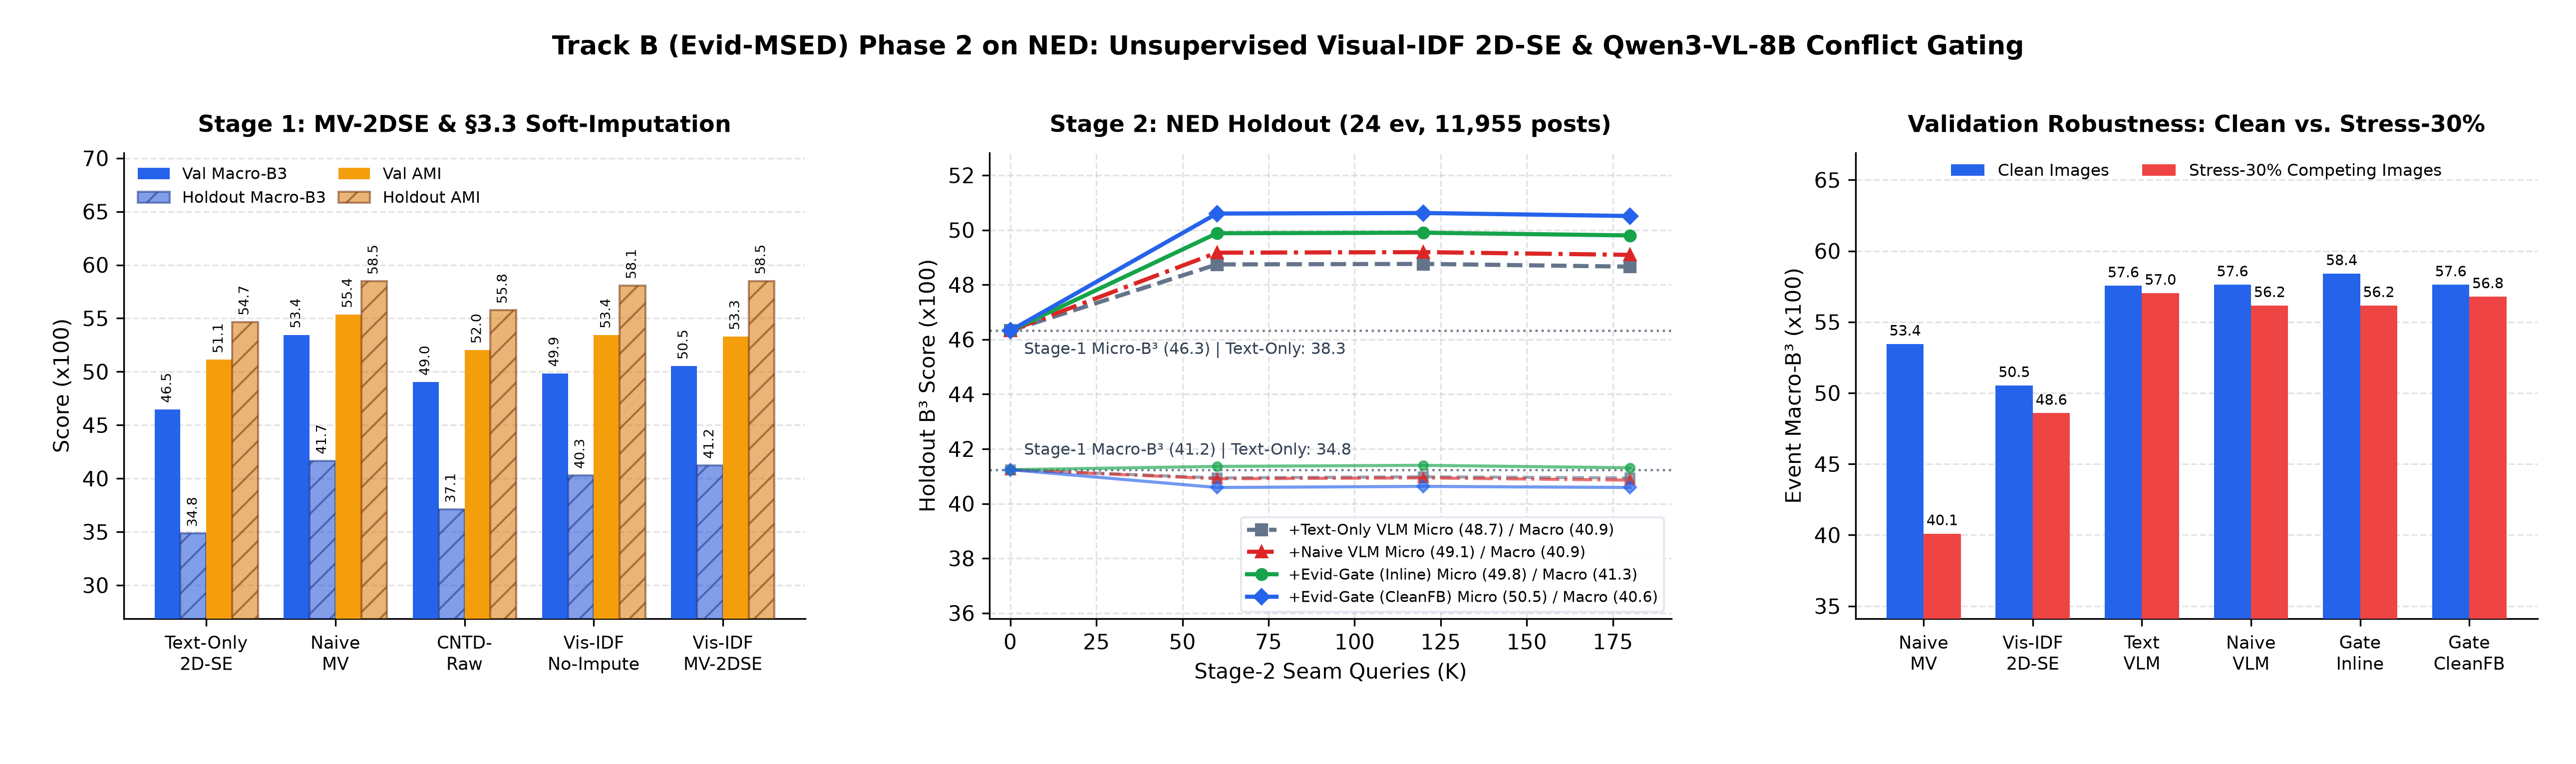
\includegraphics[width=0.98\textwidth]{figures/trackB_phase2_ned_val_holdout.png}
  \caption{Phase~2 evaluation summary: (left) Stage-1 MV-2DSE \& §\ref{sec:stage1_method} soft-imputation ablations across \texttt{Validation} and \texttt{Holdout}; (middle) Stage-2 budget trajectory ($K \in \{60, 120, 180\}$) on unseen \texttt{NED Holdout} showing strong Micro-$B^3$ progression alongside concave diminishing returns after $K=60$; (right) Clean vs.\ Stress-30\% robustness on \texttt{Validation}.}
  \label{fig:phase2_main}
\end{figure*}

\subsection{Stage 2: Conflict-Gated Seam Adjudication}
\label{sec:exp_stage2}

Table~\ref{tab:trackb_stage2_ned} and Figure~\ref{fig:phase2_main} summarize Stage~2 across Clean and Stress-30\% regimes (note \texttt{evid\_comp\_gate\_clean\_fallback} produced identical metrics to \texttt{evid\_self\_gate\_clean\_fallback} because all gated multimodal decisions already satisfied $\text{conf} \ge 0.70$):

\begin{itemize}
    \item \textbf{Clean Supremacy and Leverage:} On \texttt{Validation Clean} ($K=60$), \texttt{Evid-SelfGate (Inline)} wins across every metric---lifting AMI to $0.5748$, Macro-$B^3$ to $0.5841$ ($+7.87\text{ pp}$ over Stage~1, $+11.94\text{ pp}$ over text-only 2D-SE), Micro-$B^3$ to $0.5544$, and unqueried leverage to $19.45$ posts/call ($+1{,}167$ net improved posts vs.\ $13.25$ for \texttt{Naive VLM}). On \texttt{Holdout Clean}, \texttt{Evid-SelfGate (Inline)} is the only policy improving over Stage~1 across all aggregate metrics at both $K=60$ (AMI $0.5877$, Macro-$B^3$ $0.4136$, Micro-$B^3$ $0.4988$, ARI $0.4913$, $24.63$ Fix/Q vs.\ $12.77$ for \texttt{Naive VLM}) and $K=180$ ($4.82$ vs.\ $0.86$ Fix/Q---$5.6\times$ blind VLM efficiency---by rejecting $27.22\%$ of conflicted/non-discriminative seams, preventing $1{,}536$ blind unqueried degradations suffered by \texttt{Naive VLM}). Simultaneously, \texttt{CleanFB} achieves the highest Holdout Micro-$B^3$ ($0.5060$ at $K=60$, $+4.28\text{ pp}$ over Stage~1).
    \item \textbf{Inline Image-Anchoring Under Stress-30\%:} On \texttt{Validation Stress-30\%}, swapped images inside multimodal prompts biased \texttt{Qwen3-VL-8B}'s inline \texttt{same\_event\_text\_only} predictions ($\text{inline\_disagree} = 0$), pulling \texttt{Inline} down alongside \texttt{Naive VLM} ($0.5616$ Macro-$B^3$); image-free fallback (\texttt{CleanFB}) eliminated this anchoring and recovered to $0.5625$ AMI / $0.5678$ Macro-$B^3$ ($18.85$ Fix/Q). Conversely, on \texttt{Holdout Stress-30\%} ($K=60$), \texttt{Inline} achieved top Stress AMI ($0.5605$), Macro-$B^3$ ($0.3778$), ARI ($0.4174$), and $100\%$ merge precision ($1$ TP / $0$ FP), outperforming \texttt{Text-Only VLM} ($0.3595$, hurt by 2 small-event merge errors) by $+1.83\text{ pp}$.
    \item \textbf{Concave Budget Saturation ($K=60$ Peak):} On Holdout Clean, nearly all Stage-2 gains arrive by $K=60$ ($63{,}742$ tokens for \texttt{Inline}), while extending to $K=180$ dilutes per-query Fix/Q from $24.63$ to $4.82$.
\end{itemize}

\begin{table*}[t]
\centering
\caption{Stratified 24-Event Breakdown (\textbf{Small} $<200$ [8 events, $5.8\%$ of posts], \textbf{Medium} $200\text{--}599$ [7 events], \textbf{Head} $\ge 600$ [9 events]) and Stage-2 Executed Action Confusion Matrix on Held-Out \texttt{NED Holdout} ($11{,}955$ posts).}
\label{tab:trackb_strata_ned}
\resizebox{\textwidth}{!}{%
\begin{tabular}{llcccccc}
\toprule
\textbf{Condition} & \textbf{Method} & \textbf{Small $B^3$} & \textbf{Medium $B^3$} & \textbf{Head $B^3$} & \textbf{Macro-$B^3$} & \textbf{Merge TP/FP (Prec.)} & \textbf{Split TP/FP (Prec.)} \\
\midrule
\multirow{6}{*}{Holdout Clean}
& Text-Only 2D-SE (Stage 0) & 0.3326 & 0.3388 & 0.3703 & 0.3485 & --- & --- \\
& Vis-IDF MV-2DSE (Stage 1) & \textbf{0.3753} & 0.4006 & 0.4545 & 0.4124 & --- & --- \\
& + Text-Only VLM ($K=60$) & 0.3270 & \textbf{0.4158} & 0.4777 & 0.4094 & 4/1 (0.8000) & 5/3 (0.6250) \\
& + Naive VLM ($K=60$) & 0.3265 & 0.4135 & 0.4790 & 0.4091 & 2/2 (0.5000) & 5/3 (0.6250) \\
& + \textbf{Evid-SelfGate (Inline, $K=60$)} & 0.3272 & 0.4157 & 0.4887 & \textbf{0.4136} & 4/2 (0.6667) & 5/3 (0.6250) \\
& + Evid-SelfGate (CleanFB, $K=60$) & 0.2905 & 0.4157 & \textbf{0.5008} & 0.4059 & 5/2 (0.7143) & 5/3 (0.6250) \\
\midrule
\multirow{6}{*}{Holdout Stress-30\%}
& Naive MV-2DSE (Stage 1) & 0.3151 & 0.3025 & 0.3792 & 0.3355 & --- & --- \\
& Vis-IDF MV-2DSE (Stage 1) & 0.3564 & 0.3269 & 0.4352 & 0.3773 & --- & --- \\
& + Text-Only VLM ($K=60$) & 0.2972 & \textbf{0.3273} & \textbf{0.4400} & 0.3595 & 3/2 (0.6000) & 15/3 (0.8333) \\
& + Naive VLM ($K=60$) & 0.3567 & 0.3272 & 0.4357 & 0.3777 & 0/0 (0.0000) & 15/3 (0.8333) \\
& + \textbf{Evid-SelfGate (Inline, $K=60$)} & \textbf{0.3567} & 0.3272 & 0.4359 & \textbf{0.3778} & \textbf{1/0 (1.0000)} & 15/3 (0.8333) \\
& + Evid-SelfGate (CleanFB, $K=60$) & 0.3473 & 0.3272 & 0.4358 & 0.3746 & 1/1 (0.5000) & 15/3 (0.8333) \\
\bottomrule
\end{tabular}}
\end{table*}

\begin{figure*}[t]
  \centering
  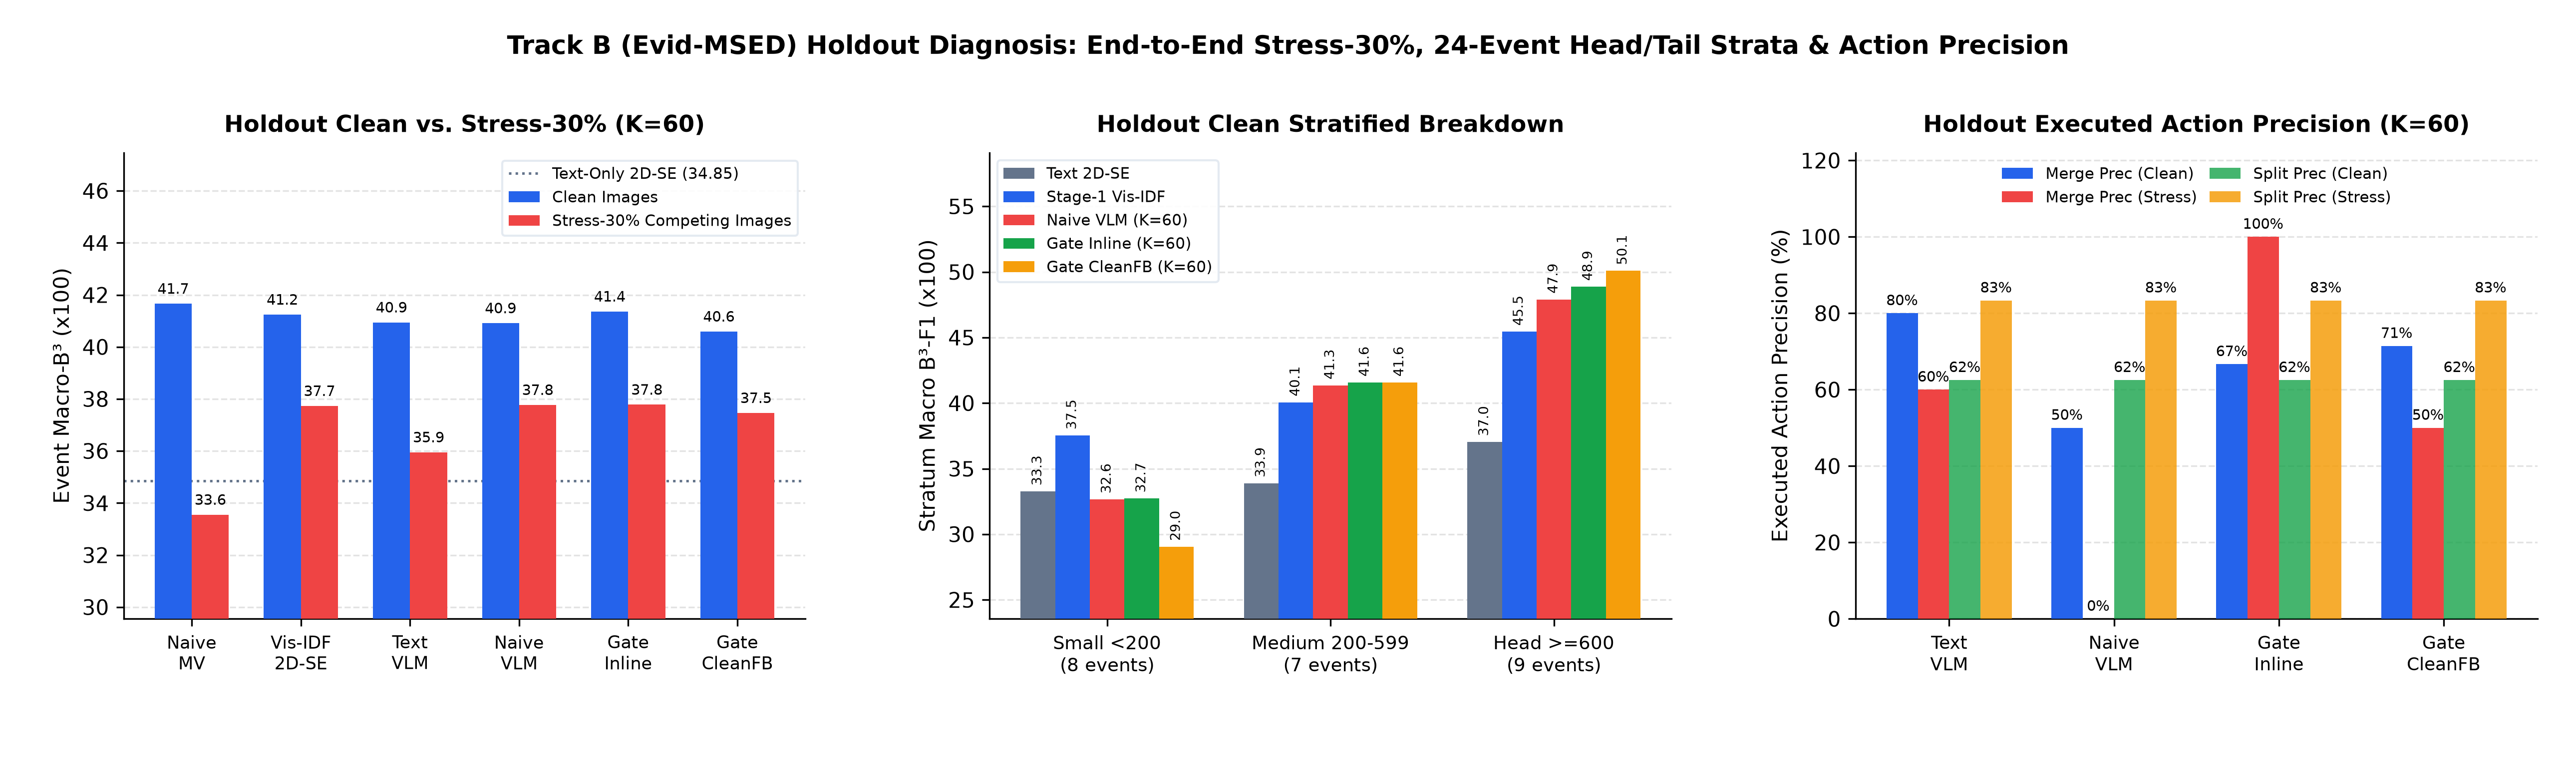
\includegraphics[width=0.98\textwidth]{figures/trackB_phase2_holdout_stress_and_strata.png}
  \caption{Holdout diagnosis ($24$ events, $11{,}955$ posts): (left) End-to-end Clean vs.\ Stress-30\% Macro-$B^3$ at $K=60$; (middle) Clean stratified breakdown showing monotonic Stage~1+Stage~2 gains on Medium and Head events ($0.3703 \to 0.5008$) vs.\ tail erosion from $2$ hard union-find merges; (right) Executed merge and split action precision.}
  \label{fig:holdout_diag}
\end{figure*}

\subsection{Why Micro-$B^3$ Rises While Macro-$B^3$ Plateaus on Holdout}
\label{sec:exp_strata}

Inspecting Stage-2 Holdout numbers superficially might suggest Stage~2 adds little beyond Stage~1 ($\Delta\text{Macro-}B^3 = +0.12\text{ pp}$ for \texttt{Inline}). Table~\ref{tab:trackb_strata_ned} and Figure~\ref{fig:holdout_diag} expose the exact mathematical mechanism:
\begin{enumerate}
    \item \textbf{Large Cumulative Gains on Head and Medium Events:} While Stage~1 elevates all three size strata uniformly (Small $+4.27\text{ pp}$, Medium $+6.18\text{ pp}$, Head $+8.42\text{ pp}$), Stage~2 further pushes Head events ($\ge 600$ posts) from $0.4545 \to 0.4887$ (\texttt{Inline}) and $0.5008$ (\texttt{CleanFB}, $+13.05\text{ pp}$ cumulative over Text-Only), driven by major true merges such as \texttt{E7} ($0.5144 \to 0.7338$, $+21.94\text{ pp}$), \texttt{E4} ($0.4308 \to 0.5552$, $+12.44\text{ pp}$), and \texttt{E37} ($0.3780 \to 0.4641$, $+8.61\text{ pp}$).
    \item \textbf{Two Size-Asymmetric Merge False Positives Erase Tail Weight:} The 8 Small events ($<200$ posts) comprise only $5.8\%$ ($697$) of posts yet carry $33.3\%$ of equal-weighted Event Macro-$B^3$. Although gating increases Holdout Clean merge precision over \texttt{Naive VLM} ($50.0\% \to 66.7\%$ \texttt{Inline} / $71.4\%$ \texttt{CleanFB}), exactly \textbf{two executed \texttt{MERGE} false positives} joined a small cluster into a giant Head cluster ($\text{stratum\_merge\_fp} = \{\text{small}:2, \text{medium}:0, \text{head}:2\}$). Under hard union-find concatenation, absorbing a $<200$-post cluster into a $500$+ post cluster collapses small-event $B^3$ precision (\texttt{E30}: $0.7420 \to 0.3780$ Inline / $0.1654$ CleanFB; \texttt{E18}: $0.4147 \to 0.1488$ Inline / $0.0932$ CleanFB), deducting enough tail points to offset Head gains inside Macro-$B^3$.
\end{enumerate}

\paragraph{Qualitative Stage-2 Seam Cases.}
Real seam logs highlight how explicit gating works on anonymized clusters: (i) \emph{Rescues:} in Validation \texttt{seam\_c32}, two pockets sharing generic \texttt{cnn} tokens split accurately when \texttt{Qwen3-VL-8B} contrasts a Scottish independence vote broadcast against nuclear-victim archival footage ($\text{conf}=1.0$); in Validation \texttt{seam\_c34}, distinct \texttt{\#nepal} emergency contacts vs.\ Google Person Finder screenshots merge cleanly; in Holdout \texttt{merge\_c56\_c90}, Hong Kong street protest schedules and street confrontations unite (\texttt{Text-Only} $= \text{False} \to \text{MM} = \text{True}$). (ii) \emph{Conflict Blocks:} Validation Stress \texttt{seam\_c3} injects a whiskey bottle photo onto sports text ($\text{vis\_conflict} = \text{True}$); Holdout Stress \texttt{merge\_c22\_c103} pairs Sri Lanka blast text with a generic prayer cluster holding a \emph{``Pray for Mexico''} flag---where \texttt{Text-Only VLM} mistakenly merges on generic prayer words while multimodal conflict gating blocks it ($\text{mm} = \text{False}$).

\section{Limitations and Conclusion}
\label{sec:conclusion}

\subsection{Limitations and Open Engineering Directions}
We highlight four candid boundaries of this work:
\begin{enumerate}
    \item \textbf{Single Multi-Event Corpus Evaluated End-to-End:} All Phase~1 and Phase~2 results are measured on \texttt{NED}~\cite{lin2024ned}. While we eliminated \texttt{NED}'s 72-hour chronological shortcut and enforced strict unseen 24-event holdout evaluation, cross-lingual generalization to Chinese multimodal streams (\texttt{WEIBO2022}~\cite{han2026kqgnn}) or real same-day natural disaster pairs (\texttt{CrisisMMD}~\cite{alam2018crisismmd}) remains to be validated once raw visual assets are available locally.
    \item \textbf{Sensitivity of Hard Union-Find to Size-Asymmetric Merges:} Our stratified audit pinpoints that two Small$\leftrightarrow$Head \texttt{MERGE} false positives drive tail $B^3$ erosion under direct union-find merging. Guarding \texttt{MM\_MERGE\_PAIR} decisions when $|C_a| / |C_b| > 4$ via weighted graph edge addition and bounded 2D-SE re-clustering---rather than unconditional union-find---offers a principled fix without sacrificing Head gains.
    \item \textbf{Inline Image-Anchoring in 8B VLMs:} On \texttt{Validation Stress-30\%}, exposing \texttt{Qwen/Qwen3-VL-8B-Instruct} to corrupted images contaminated its inline text-only judgment field; decoupling image-free text fallback (\texttt{CleanFB}) cures anchoring but costs extra fallback tokens.
    \item \textbf{Single VLM Backbone:} We audited one open-weight 8B VLM (\texttt{Qwen/Qwen3-VL-8B-Instruct}); comparative cross-backbone evaluation with larger VLMs is left for future work.
\end{enumerate}

\subsection{Conclusion}
We investigated when images genuinely disambiguate social events versus when they cause cross-event false merges once calendar separation shortcuts are removed. Through a paired counterfactual causal audit on concurrent \texttt{NED} splits, we empirically refuted static caption-dispersion filtering (\texttt{CNTD-Raw}) and established that graph-level redundancy suppression (\texttt{Visual-IDF}) and prompt-level cross-modal conflict gating (\texttt{visual\_discriminative} $\wedge \neg\texttt{visual\_conflict\_with\_text}$) solve complementary failure regimes. Combining Stage-1 \texttt{Visual-IDF MV-2DSE} (with corrected missing-modality soft imputation removing the degenerate $\delta_i \delta_j$ product) and Stage-2 conflict-gated mesoscopic seam adjudication on \texttt{Qwen/Qwen3-VL-8B-Instruct}, \textbf{Evid-MSED} delivers strong clustering gains over text-only 2D-SE on unseen 24-event streams ($+3.84\text{ pp}$ AMI, $+6.38\text{ pp}$ Macro-$B^3$, $+8.02\text{ pp}$ Micro-$B^3$ in Stage~1; reaching $0.5060$ Micro-$B^3$ and $24.63$ net fixed unqueried posts per query at $K=60$ in Stage~2), prevents naive multimodal collapse under $30\%$ competing-image corruption, and supplies a transparent head/medium/tail roadmap for safer mesoscopic multimodal graph editing.


\bibliographystyle{ACM-Reference-Format}
\bibliography{references}

\clearpage
\appendix
\section{Prompt Schemas and Frozen Protocol}
\label{sec:appendix}

\subsection{Anonymized Dual-Image Seam VLM Prompts}
Across all Gate~B and Phase~2 calls to \texttt{Qwen/Qwen3-VL-8B-Instruct}, inputs never contain ground-truth \texttt{event\_name} labels or calendar years/dates. In Phase~2 Stage~2 multimodal seam queries, up to two labeled Visual-IDF representative images (\texttt{"Representative Image for Cluster A:"} and \texttt{"Representative Image for Cluster B:"}) are passed alongside anonymized cluster briefs (top-5 hashtags/tokens and up to 3 medoid tweets clipped at $145$ characters). The model is constrained to \texttt{response\_format=json\_object} with explicit fields:
\begin{verbatim}
{
  "event_a": "<5-10 words>",
  "event_b": "<5-10 words>",
  "visual_clue_a": "<5-10 words or none>",
  "visual_clue_b": "<5-10 words or none>",
  "visual_discriminative": true | false,
  "visual_conflict_with_text": true | false,
  "same_event_text_only": true | false,
  "same_event_multimodal": true | false,
  "evidence_source": "text"|"image"|"both"|"none",
  "confidence": <float in [0.0, 1.0]>
}
\end{verbatim}
In \texttt{text\_only} mode (used for \texttt{text\_only\_vlm} and \texttt{CleanFB} fallback), images and visual fields are omitted and the prompt returns \texttt{\{"event\_a", "event\_b", "same\_event", "confidence"\}}.

\subsection{Frozen Protocol Hyperparameters}
Table~\ref{tab:protocol_trackb} archives all immutable Stage~1, Stage~2 router, and VLM hyperparameters recorded in \texttt{trackB\_evid\_msed/protocol\_trackB\_v1.json} prior to unlocking the 24-event \texttt{NED Holdout} split.

\begin{table}[h]
\centering
\caption{Exact Frozen Hyperparameters in \texttt{protocol\_trackB\_v1.json} (Locked Prior to Unseen \texttt{NED Holdout} Execution).}
\label{tab:protocol_trackb}
\resizebox{\columnwidth}{!}{%
\begin{tabular}{ll}
\toprule
\textbf{Component / Parameter} & \textbf{Frozen Value} \\
\midrule
Protocol Version & \texttt{Evid-MSED-v1.0-frozen} (\texttt{2026-11-22T15:30:01Z}) \\
Frozen SHA-256 Tracked Files & 9 Python modules (\texttt{core\_shared/*}, \texttt{trackB\_evid\_msed/*}) \\
Text Encoder & \texttt{sentence-transformers/all-MiniLM-L6-v2} ($384$-d) \\
Visual Encoder & \texttt{openai/clip-vit-base-patch32} ($512$-d, center-crop bicubic) \\
Text Graph $W^T$ & $\text{knn\_k}=12$, $\theta_T=0.38$, $\alpha=0.45$, $\lambda_\tau=0.0$ \\
Stage-1 Visual-IDF Weighting & \texttt{block\_size}$=1{,}024$, near-dup $\cos \ge 0.88$ \\
§\ref{sec:stage1_method} Soft Imputation & $\tau_{\text{imp}}=0.55$, $\gamma_{\text{imp}}=0.70$, \texttt{use\_soft\_imputation}=\texttt{True} \\
Visual View $W^V$ & $k_V=10$, $\theta_V=0.72$, $\lambda_V=0.65$ \\
2D-SE Solver & Exact greedy agglomerative + monotone node-move refine \\
Stage-2 Router & $K=180$ (prefixes $60/120/180$), $\rho_M=0.70$, $\tau_{\text{conf}}=0.60$ \\
Merge Candidate Gate & $t_{\text{sim}} \ge 0.42$ ($\text{cut}\ge 2.0$) $\vee$ ($v_{\text{sim}}\ge 0.68 \wedge t_{\text{sim}}\ge 0.18 \wedge \text{vidf}\ge 0.50$) \\
Seam Detector Gate & $|C|\ge 10$, $|S_p|\ge 4$, conductance $\le 0.50$, $\Delta_{\text{sem}} \ge 0.08$ \\
VLM Endpoint & \texttt{Qwen/Qwen3-VL-8B-Instruct} (SiliconFlow, $\text{temp}=0.0$) \\
Image Payload & Max side $384\text{px}$ JPEG ($q=82$), SHA-256 hash cache \\
\bottomrule
\end{tabular}}
\end{table}


\end{document}
